\documentclass[final,3p, review, times]{Elsevier/elsarticle}

%% ------ Custom Packages -----------
\usepackage{etex}
\usepackage{amsmath}
\allowdisplaybreaks
\usepackage{amssymb}
\usepackage{amsthm}
\usepackage{xcolor}
\usepackage{fancyvrb}
\usepackage{hyperref}
\usepackage{graphicx}
\usepackage{listings}
\usepackage{titlesec}
\usepackage{paralist}
\usepackage{multirow}
\usepackage{calc}
\usepackage{tocloft}
\usepackage{pstricks,pst-node,pst-tree,pstricks-add}  %% for drawing CFG and 2D view of the lattice
\usepackage{tikz}  %% for drawing rest of the images
\usetikzlibrary{shapes, snakes, decorations.markings}
\tikzset{
  ->-/.style={
    thick,
    postaction = {decorate},
    decoration = {
      markings,
      mark = at position #1 with {
        \arrow{stealth}
      }
    }
  },
  ->-/.default = 0.5
}
\tikzset{
  -<-/.style={
    thick,
    postaction = {decorate},
    decoration = {
      markings,
      mark = at position #1 with {
        \arrow{stealth reversed}
      }
    }
  },
  -<-/.default = 0.5
}

%% ------ Custom Commands -----------
\makeatletter
\newcommand{\op}[3][\@empty]{
  \ifx\@empty#1\relax
    \ \tikz[baseline=(char.base)]{
      \node[shape=circle,draw,inner sep=0pt] (char) {$\mathtt{{#2}_{#3}}$};
    }\ 
  \else
    \ \tikz[baseline=(char.base)]{
      \node[shape=circle,draw,fill=black!90,text=white,inner sep=0pt] (char) {$\mathtt{{#2}_{#3}}$};
    }\ 
  \fi
}
\makeatother
\newlength{\depthofsumsign}
\setlength{\depthofsumsign}{\depthof{$\sum$}}
\newcommand{\nsum}[1][1.4]{
  \mathop{
    \raisebox{
      -#1\depthofsumsign+1\depthofsumsign
    }{
      \scalebox{#1}{$\displaystyle\sum$}
    }
  }
}
\titleformat*{\section}{\Large}
\newcommand{\ALPHA}{\large\boldsymbol{\alpha}\normalsize}
\newcommand{\GAMMA}{\large\boldsymbol{\gamma}\normalsize}
\def\checkmark{\tikz\fill[scale=0.4](0,.35) -- (.25,0) -- (1,.7) -- (.25,.15) -- cycle;}
\renewcommand{\cftsecleader}{\cftdotfill{\cftdotsep}}

\hypersetup{
  pdfstartview = {FitH},
  pdffitwindow = true,
  pdfnewwindow = true,
  colorlinks   = true,
  urlcolor     = blue,
  linkcolor    = blue,
  citecolor    = cyan,
  pdfauthor    = {Dibyendu Das},
  pdfcreator   = {LaTeX},
  pdfkeywords  = {Interval Analysis, Static Analysis, Abstract Interpretation, Probabilistic Programming Language},
  pdftitle     = {Interval Analysis of Unreliable Programs},
  pdfsubject   = {Research Thesis},
  pdfpagemode  = UseNone
}
%% ------------------------------

\newtheorem{theorem}{Theorem}[section]
\newtheorem{definition}{Definition}[section]

\begin{document}

\title{
{--------------------------------------------------------------------}\\
{Interval Analysis of Unreliable Programs}\\
{--------------------------------------------------------------------}\\
{\large A thesis submitted in partial fulfillment of\\
The requirements for the degree of Master of Technology\\
in\\
Computer Science and Engineering\\}
}
\author{By\\
Dibyendu Das\\
Roll No. 14CS60R34\\
Under the supervision of\\
Prof Soumyajit Dey\\
Dept. of CSE, IIT Kharagpur\\~\\

\includegraphics[width=5cm]{logo.jpg}\\
Department of Computer Science and Engineering\\
Indian Institute of Technology, Kharagpur}
\maketitle
\clearpage

\tableofcontents

\clearpage
\phantomsection
\chapter{\LARGE\begin{center}Certification\end{center}}
{\large
This is to certify that the project entitled "\textit{Interval Analysis of Unreliable Programs}" being submitted by Dibyendu Das is a bonafide work done by him in the Department of Computer Science and Engineering, Indian Institute of Technology, Kharagpur under my supervision and guidance for M.Tech Project.}\\~\\~\\~\\~\\~\\~\\~\\~\\~\\~\\~\\~\\~\\~\\~\\~\\~
\begin{flushright}
---------------------------------------------------------------------\\~\\~
Prof. Soumyajit Dey \\~
Department of Computer Science and Engineering\\~
IIT Kharagpur\\~
\end{flushright}

\clearpage
\phantomsection
\chapter{\LARGE\begin{center}Declaration\end{center}}
{\large
This thesis is a presentation of my original research work. Wherever contributions of others are involved, every effort is made to indicate this clearly, with due reference to the literature and acknowledgement of collaborative researchand discussions. The work was done under the guidance of Prof. Soumyajit Dey, at Indian institute of Technology, Kharagpur.}\\~\\~\\~\\~\\~\\~\\~\\~\\~\\~\\~\\~\\~\\~\\~\\~\\~
\begin{flushright}
---------------------------------------------------------------------\\~\\~
Dibyendu Das\\~
Department of Computer Science and Engineering\\~
IIT Kharagpur\\~
\end{flushright}

\clearpage
\phantomsection
\chapter{\LARGE\begin{center}Acknowledgements\end{center}}
{\large This thesis is the result of the project work performed under the guidance of Prof. Soumyajit Dey at the Department of Computer Science and
Engineering of the Indian Institute of Technology, Kharagpur. I am deeply grateful to my supervisor for having given me the opportunity of working under him and guiding me seamlessly for the whole period. He gave me exposure to all the related research going on in this field, which helped me enormously. Without the help, encouragement and patient support I received from my guide, this report would never have materialized.}\\~\\~\\~\\~\\~\\~\\~\\~\\~\\~\\~\\~\\~\\~\\~\\~\\~
\begin{flushright}
---------------------------------------------------------------------\\~\\~
Dibyendu Das\\~
Department of Computer Science and Engineering\\~
IIT Kharagpur\\~
\end{flushright}

\clearpage
\phantomsection
\chapter{\LARGE\begin{center}Abstract\end{center}}
Advancement of chip technology will make futute computer chips more and more fast. But this speed gain doesn't come free of cost. There is going to be a trade-off between speed and efficiency, i.e accuracy of the computation. In order to achieve this extra speed we'll simply have to let our computers make more mistakes in computations. Consequently systems built with these type of chips will possess an innate unreliability lying within. Programs written for these systems will also have to incorporate this unreliability. Researchers have already started developing programming frameworks\cite{carbin13} for unreliable architectures as such.

In this paper, we have used a restricted version of C-type languages to model the programs written for this architecture. We, here, propose a technique for statically analysing codes written for these kind of architecture. Our technique, which primarily focuses on \textit{Interval/Range Analysis} of this type of programs, uses the well established method of \textit{Abstract Interpretation}. While discussing unreliability of hardware, there comes scope of failure of the hardware components implicitly. There are 2 types of failure models, namely: \emph{permanent failure model}, where the hardware stops execution on failure and \emph{transient failure model}, where on failure, the hardware continues to work with the subsequent operations. In this paper, we've only taken transient failure model into consideration. The goal of this analysis is to be able to predict, \textbf{for each program variable, at each program point, the interval/range within which it belongs and the safe probability of belonging}. Say for example, for program with $n$ variables namely $x_1,x_2\cdots x_n$, this analysis will produce output like $x_i=\langle[a,b],p_{ab}\rangle$ for each $i$, at every program point. This means that variable $x_i$, at that program point lies in the interval $[a,b]$ with probability $p_{ab}$.

The major applications or this work can be \emph{calculating the success probability of the overall program}, \emph{static branch prediction} for such languages. Other application could be \emph{detection of most reliable path in the program}.
\clearpage



\section{Introduction}

As transistors approach sub-atomic sizes, reliability is increasingly jeopardized. The smaller it gets, the less reliable it becomes. Computer-chip designers keep figuring out technical workarounds to the miniaturization problem; however, prevailing wisdom maintains that current manufacturing techniques will sooner or later run out of steam, and Moore’s Law -- the prediction that has yielded huge increases in semiconductor performance for nearly five decades -- will be no more. So far, the chip designers have been able to work around that problem, but in the future, it could mean that computers stop improving at the rate we’ve come to expect.

Researchers are scrambling to come up with alternatives to silicon-based CMOS, but some scientists are suggesting another possibility: \emph{let the computers make mistakes}. We could simply let our computers make more mistakes. Computational reliability won't be a major issue in some cases. If, for instance, a few pixels in each frame of a high-definition video are improperly decoded, viewers probably won’t notice --- but relaxing the requirement of perfect decoding could yield gains in speed or energy efficiency.

Emerging high-performance architectures are anticipated to contain unreliable components that may exhibit soft errors, which silently corrupt the results of computations. While full detection and masking of soft errors is challenging, expensive, and, for some applications, unnecessary, some applications can withstand a certain amount of errors. For example, approximate computing applications such as
\begin{inparaenum}[\itshape i\upshape)]
  \item Multimedia processing,
  \item High definition video decoding,
  \item Image manipulation,
  \item Machine learning,
  \item Big data analytics
\end{inparaenum}
can often naturally tolerate soft errors.

Works have already been done on modelling and manufacturing unreliable hardware components. Probabilistic CMOS or PCMOS technology yield several orders of magnitude improvements in terms of energy over conventional (deterministic) CMOS based implementations\cite{chakrapani08}. Foundational principles of PCMOS technology is used to build probabilistic switchs, which are in turn used to realize FIR filter used in the H.264 decoding algorithm\cite{marpe05}. Stochastic Processors are also there, that tolerate hardware errors while producing outputs that are, in the worst case, stochastically correct. People have built programmable analog computer based on a regular array of stochastic computing element logic\cite{rascel69}.

There has been work done on software level too. For handling the (future) unreliable chips, researchs at MIT's Computer Science and Artificial Intelligence Laboratory (CSAIL) have developed a new programming framework called RELY\cite{carbin13} that enables software developers to specify when errors may be tolerable. The system then calculates the probability that the software will perform as it's intended.

In this report, we present a static analysis technique called \textbf{Range Analysis} or \textbf{Interval Analysis} for unreliable programs written for these type of unreliable hardware. We call it \textbf{Probabilistic Interval Analysis}. Our approach takes into count, the unreliabilities that occur because of ALU and Memory operations generally found in all high level programming languages.

\section{Objective}

We propose a general abstract interpretation based method for the static analysis of programs that run on unreliable hardwares. Our method does Interval analysis for programs like these. The objectibe is to calculate the success probability of the overall program and other similar tasks like detecting the most reliable path in the program.

More formally, for a program with $n$ integer variables, we are interested in answering questions like, with what probability does each program variable lie in a range of values at each program point. In other words, goal is to find out the probability that $x_i\in[a,b]$ at program point $p_i$.

\section{Related Work}

There have already been some work on static analysis of programs with \emph{imprecise probabilistic inputs} \cite{vstte13}, which heavily relies on Dempster-Shafer structures (DSI) or P-boxes. This analyzer assumes each input value to be lying within a \textit{confidence box} $[\underline{P},\overline{P}]$. Based on this assumption it works on to perform the interval analysis of each variable at each program point. Few other works are there, where people analyze programs with non-deterministic and probabilistic behavior \cite{monn01}\cite{sumit13}. Those use general abstract interpretation based method for the static analysis of programs using random generators or random inputs and also allow non-deterministic inputs, not necessarily following a random distribution.

Our work is orthogonal to all these as we're concerned with the imprecision seeded into the hardware rather than in input. So, in our case inputs come from reliable sources with fully reliable values.

\section{Motivation}


\section{Unreliable Programs}

Following is an example program snippet and its corresponding \textbf{C}ontrol \textbf{F}low \textbf{G}raph of a program written for an unreliable system in which every operation (ALU or memory) is unreliable.\\

\begin{minipage}[b]{0.40\linewidth}
\centering
\begin{lstlisting}[mathescape]
//$v_0$
x $=_\bullet$ 0
//$v_1$
while (x $<_\bullet$ 10) // $v_2$
    x $=_\bullet$ x $+_\bullet$ 3
//$v_3$
\end{lstlisting}
\end{minipage}
\rule[42mm]{4mm}{.1pt}\rule[-2.5mm]{1pt}{50mm}\rule[42mm]{4mm}{.1pt}\raisebox{41.2mm}{$>$ CFG}
\hspace{0.2\linewidth}
\begin{minipage}[b]{0.40\linewidth}
$
\psmatrix[colsep=2.5cm,rowsep=1.5cm,mnode=circle]
v_0\\
v_1&v_3\\
v_2
\psset{arrowscale=2}
\everypsbox{\scriptstyle}
\ncline{->}{1,1}{2,1}>{x\ =_\bullet\ 0}
\ncline{->}{2,1}{2,2}^{x\ \geq_\bullet\ 10}
\ncline{->}{2,1}{3,1}>{x\ \leq_\bullet\ 9}
\ncarc[arcangle=-45]{<-}{2,1}{3,1}<{x\ =_\bullet\ x\ +_\bullet\ 3}
\endpsmatrix
$
\end{minipage}

\centerline{Figure 1: Example program.}

Here each operation is probabilistic i.e each operation produces correct values with some probability. Unreliable operators are denoted by the corresponding operator followed by a \textit{subscript bullet} ($\bullet$). Each operator has a success probability associated with it i.e the operator succeeds and produces correct result with a predefined probability. These probability values are set by the hardware manufacturer of the chip. Upon failure the probabilistic operators take random values from their corresponding domains. For arithmetic operators this domain is $\mathbb{Z}\cap[\mathtt{MININT},\mathtt{MAXINT}]$, for boolean operators it is $\{true, false\}$ etc. Success and corresponding failure probabilities of some of the operators are given in Table~\ref{hw-spec}.

\begin{table}
  \caption{Hardware Probability Specification}
  \begin{tabular}{@{\hspace{5mm}}c@{\hspace{1cm}}c@{\hspace{1cm}}c@{\hspace{1cm}}l@{}}
   \hline
   \multirow{2}{*}{Operator} & Probability of successful execution & \multirow{2}{*}{Failure probability} & \multirow{2}{*}{Domain of operation} \\
   & (given by hardware manufacturer) & & \\
   \hline
   $+_\bullet$ & $Pr(+_\bullet)$ & $1-Pr(+_\bullet)$ & \multirow{5}{*}{$\big\{a\in\mathbb{Z}\ |\ \mathtt{MININT}\leq a\leq\mathtt{MAXINT}\big\}$} \\
   $-_\bullet$ & $Pr(-_\bullet)$ & $1-Pr(-_\bullet)$ & \\
   $\times_\bullet$ & $Pr(\times_\bullet)$ & $1-Pr(\times_\bullet)$ & \\
   $\div_\bullet$ & $Pr(\div_\bullet)$ & $1-Pr(\div_\bullet)$ & \\
   $=_\bullet$ & $Pr(Wr)$ & $1-Pr(Wr)$ & \\
   \hline
   $>_\bullet$ & $Pr(>_\bullet)$ & $1-Pr(>_\bullet)$ & \multirow{2}{*}{$\big\{true,\ false\big\}$} \\
   $\geq_\bullet$ & $Pr(\geq_\bullet)$ & $1-Pr(\geq_\bullet)$ & \\
   \hline
   $\vdots$ & $\vdots$ & $\vdots$ & \\
  \end{tabular}
  \label{hw-spec}
\end{table}

For example, this program statement \\ \centerline{$\sigma : x\ =_\bullet\ x\ +_\bullet\ 3$} \\ involves 3 probabilistic operations namely Read (\textbf{Rd}) of the variable $x$, Add (\textbf{+}) \& Write (\textbf{Wr}) to the variable $x$. So, the probability that $\sigma$ executes successfully is $\quad Pr(Rd)\cdot Pr(+_\bullet)\cdot Pr(Wr)$. Now we compute the probability with which program variable $x$ holds correct value after the execution of $\sigma$.

These three operations are independent of each other. Corresponding to three operations we have three events namely:

\begin{itemize}
\item A: \textbf{Read} executes successfully.
\item B: \textbf{Add} ($+_\bullet$) executes successfully.
\item C: \textbf{Write} executes successfully.
\end{itemize}
\[ \therefore\qquad Pr(A)=Pr(Rd),\quad Pr(B)=Pr(+_\bullet)\quad\mathrm{and}\quad Pr(C)=Pr(Wr) \]
All three events are pairwise independent but none of them are mutually exclusive.\\

\def\firstcircle{(0,0) circle (1.5cm)}
\def\secondcircle{(60:2cm) circle (1.5cm)}
\def\thirdcircle{(0:2cm) circle (1.5cm)}
\centerline{
\begin{tikzpicture}
\begin{scope}[shift={(3cm,-5cm)}, fill opacity=0.5]
\fill[gray] \firstcircle;
\fill[lightgray] \secondcircle;
\fill[white] \thirdcircle;
\draw \firstcircle node[below left] {$A$};
\draw \secondcircle node [above] {$B$};
\draw \thirdcircle node [below right] {$C$};
\end{scope}
\end{tikzpicture}
}

After $\sigma$ is executed the variable $x$ will hold the desired value with probability
\begin{multline}
  Rel_{cur}(x) = Rel_{prev}(x)\cdot\left(Pr(Rd) + \frac{1-Pr(Rd)}{\mathtt{MAXINT}-\mathtt{MININT}+1}\right)\cdot\left(Pr(+_\bullet) + \frac{1-Pr(+_\bullet)}{\mathtt{MAXINT}-\mathtt{MININT}+1}\right)\cdot \\ \left(Pr(Wr) + \frac{1-Pr(Wr)}{\mathtt{MAXINT}-\mathtt{MININT}+1}\right) \nonumber
\end{multline}
Where, $Rel_{prev}(x)$ is the probability with which variable $x$ holds the correct value just before this statement is executed.

We are interested in static analysis of these type of probabilistic programs by employing the theory of Abstract Interpretation\cite{lara13}. Abstract Interpretation deals with two different domains of program states namely the \emph{Concrete Domain}, $\mathcal{L}$ and the \emph{Abstract Domain}, $\mathcal{M}$ and a pair of connections between them namely the \emph{Galois Connection (GC)}. The Concrete Domain is a set of all possible concrete program states, where each concrete program state holds the set of all possible values a particular program varible can take during execution of the program. On the other hand, the Abstract Domain is the set of all possible abstract program states. An abstract program state is the abstraction of one concrete program state. In case of Interval Abstraction it is a range of values, a particular program varible can take during execution.

\section{The Probabilistic Concrete Domain, $\mathcal{L}:(L,\sqsubseteq_L)$}

From the above arguments we can infer that in the concrete domain each possible program state is associated with some probability. We represent program state as a tuple of sets values and its associated probability. For program with a single integer variable, we difine the concrete domain, $L\subseteq2^{\mathbb{Z}}\times\mathbb{R}$, as
\begin{definition}
$L=\left\{\left(S\in2^{\mathbb{Z}},\ p\in\mathbb{R}\right)\ \middle|\ S\neq\phi\bigwedge\forall s\in S, \mathtt{MININT}\leq s\leq\mathtt{MAXINT}\bigwedge 0\leq p\leq1\right\}\bigcup\left\{\left(\phi,1\right)\right\}$
\end{definition}

Throughout our discussion we assume that our program variables take values between $\mathbf{\mathtt{MININT}}$ and $\mathbf{\mathtt{MAXINT}}$ (including both). $\langle S_i,p_i\rangle$ denotes that at a particular program point, say $v_i$, variable $x_i$ (say) takes its values from set $S_i$ with probability $p_i$. In general, for program with $n$ integer variables, this concrete domain will be $L^n$. We define a partial order $\sqsubseteq_L$ on $L$ as follows :
\begin{definition}\label{concrete_order}
$\forall \langle S_1,p_1\rangle, \langle S_2,p_2\rangle\in L\qquad\langle S_1,p_1\rangle\sqsubseteq_L \langle S_2,p_2\rangle\quad\iff \quad S_1\subseteq S_2\ \bigwedge\ p_1\geq p_2$
\end{definition}
As an example,
\[ \langle\{a_1, a_2,\cdots a_n\},p_1\rangle\sqsubseteq_L\langle\{a_1, a_2,\cdots a_m\},p_2\rangle\quad\text{iff}\quad n\leq m, \text{so that\ }\{a_1,a_2\cdots a_n\}\subseteq\{a_1,a_2\cdots a_m\}\quad\&\quad p_1\geq p_2 \]

$(L,\ \sqsubseteq_L)$ is a \textbf{poset}, proof of which is given in \ref{app:concrete_partial}. To show this poset to be a \textbf{lattice}, we need to show that for any two elements in $L$ there exist a unique infimum and a unique supremum. More formally,
\begin{multline*}
  \forall x,y\in L\ \ \Bigg( \\
  \quad\exists L_{lub}\in\Big\{u\in L\ \ \big|\ \ (x\sqsubseteq_L u)\land(y\sqsubseteq_L u)\Big\}\ s.t\ \bigg(\forall z\ \ \Big(z\in\Big\{u\in L\ \ \big|\ \ (x\sqsubseteq_L u)\land(y\sqsubseteq_L u)\Big\} \Rightarrow L_{lub}\sqsubseteq_L z\Big)\bigg) \\
  \hfill\bigwedge\hfill \\
  \quad\exists L_{glb}\in\Big\{l\in L\ \ \big|\ \ (l\sqsubseteq_L x)\land(l\sqsubseteq_L y)\Big\}\ s.t\ \bigg(\forall z\ \ \Big(z\in\Big\{l\in L\ \ \big|\ \ (l\sqsubseteq_L x)\land(l\sqsubseteq_L y)\Big\} \Rightarrow z\sqsubseteq_L L_{glb}\Big)\bigg) \\
  \quad\qquad\qquad\Bigg)\hfill
\end{multline*}

where $L_{lub}$ is the least upper bound and $L_{glb}$ is the greatest lower bound of $x$ and $y$ in $L$. The least upper bound $(l.u.b)$ operator, $\displaystyle\bigsqcup_L$ and the greatest lower bound $(g.l.b)$ operator, $\displaystyle\bigsqcap^L$ for any two elements $A$ and $B$ of $L$ come from Definition~\ref{concrete_order} and are as follows :

\begin{align}
  \langle S_1,p_1\rangle\ \bigsqcup_L\ \langle S_2,p_2\rangle\quad=\quad&\left\langle S_1\bigcup S_2, \textbf{min}(p_1,p_2)\right\rangle&\label{eq:lub_L}\\
  \langle S_1,p_1\rangle\ \bigsqcap^L\ \langle S_2,p_2\rangle\quad=\quad&\left\langle S_1\bigcap S_2, \textbf{max}(p_1,p_2)\right\rangle&\label{eq:glb_L}
\end{align}

Soundness of these definitions is proved in \ref{app:concrete_ub}. Greatest and least element of this lattice $(L,\ \sqsubseteq_L)$ are $\top_L$ and $\bot_L$ respectively, where

$
\top_L=\langle\{a\in\mathbb{Z}\ :\ \mathrm{MININT}\leq a\leq\mathrm{MAXINT}\}, 0\rangle \\
\indent\bot_L=\langle\{\ \}, 1\rangle
$

\noindent The \textbf{Hasse Diagram} of lattice $(L,\sqsubseteq_L)$ can be found in \ref{app:concrete_hasse}. $\forall S\subseteq L,\quad S$ has a unique $l.u.b$ and $g.l.b$ in $L$. Hence $L$ is a complete lattice.

Next, we shall define a function on $L^n$ called the \textit{strongest post-condition function}\cite{lara13}. Consider $P$ to be a predicate defined over program variables. Alternatively, we can also think of $P$ as a set of possible program states which satisfy the relation $P$. For example, $p=\langle\{5\},p_1\rangle\equiv[x=5]$ is a program state ($p_1$ is a place-holder here) and $P:[x>10]$ is a predicate such that $p\notin P$. Similarly, consider a program with three integer variables $x,\ y$ and $z$ such that $p=\langle(\{5\},p_1),(\{10\},p_2),(\{10\},p_3)\rangle\equiv[x=5,\ y=10,\ z=10]$ and $p'=\langle(\{15\},p_1),(\{0\},p_2),(\{1\},p_3)\rangle\equiv[x=15,\ y=0,\ z=1]$ are two program states ($p_1,p_2,p_3$ are place-holders here). Given a predicate $P:[x+y\geq z]$, we may observe that both $p,p'\in P$. Let $P$ denote a (pre-condition) predicate which is true before the execution of some program statement $S$. Strongest post condition (sp) is a function which takes as argument a program statement $S$ (or a sequence of statements) and a predicate $P$ and returns the strongest predicate that holds after executing $S$ from any program state which satisfies $P$. It is strongest in the sense that for any other such predicate $Q$ which holds for any state resulting from execution of $S$ given $P$, we shall always have $sp(P,S)\Rightarrow Q$ (implies $Q$) or in a set theoretic notation $sp(P,S)\subseteq Q$. As example, we consider next arithmetic expressions (with assignment) and logical expressions as examples of $S$.

We assume that there are $n$ variables in the program, namely, $x_1,x_2\cdots x_n$. At any program point, a predicate with $n$ variables will be of the form $P:\langle(S_1,p_1),(S_2,p_2),\cdots,(S_n,p_n)\rangle$, s.t at that program point each $x_i$ will have values from the set $S_i$ with probability $p_i$. Now, we define the strongest post-condition operations for arithmetic and logical expressions. In the following definitions,
\begin{flalign}
  &\mathcal{V}\Big((v_1,v_2,\cdots,v_n),x_i\Big)=\begin{cases}
      v_i       & \quad \text{if } x_i \text{ is a variable}\\
      x_i=C  & \quad \text{if } x_i \text{ is a constant, say } C\\
  \end{cases}\qquad
  \mathcal{P}(P,x_i)=\begin{cases}
      p_i       & \quad \text{if } x_i \text{ is a variable}\\
      1  & \quad \text{if } x_i \text{ is a constant}\\
  \end{cases}&&&\nonumber\\
  &\forall i,\quad\op[prob]{A}{i} \text{ is a probabilistic arithmetic operation}\quad\text{and}\quad\op{A}{i} \text{ is a deterministic arithmetic operation.}&&&\nonumber\\
  &\text{i.e}\quad\op[prob]{A}{i}\in\{+_{\bullet},-_{\bullet},\times_{\bullet},\div_{\bullet},\%_{\bullet},\cdots\}\quad\op{A}{i}\in\{+,-,\times,\div,\%,\cdots\}&&&\nonumber\\
  &\op[prob]{C}{} \text{ is a probabilistic comparison operation}\quad\text{and}\quad\op{C}{} \text{ is a deterministic comparison operation.}&&&\nonumber\\
  &\text{i.e}\quad\op[prob]{C}{}\in\{<_{\bullet},>_{\bullet},\geq_{\bullet},\leq_{\bullet},==_{\bullet},\neq_{\bullet}\}\quad\op{C}{}\in\{>,<,\geq,\leq,==,\neq\}&&&\nonumber
\end{flalign}
\begin{definition}\label{sp_arith}
  \begin{flalign}
    &\quad sp\Big(P,\ x_{i_f} =_\bullet x_{i_1} \op[prob]{A}{2} x_{i_2} \op[prob]{A}{3} \cdots \op[prob]{A}{k} x_{i_k}\Big)&&&\nonumber\\
    =&\quad sp\Big(\langle(S_1,p_1),(S_2,p_2),\cdots,(S_{i_f},p_{i_f}),\cdots,(S_n,p_n)\rangle,\ x_{i_f} =_\bullet x_{i_1} \op[prob]{A}{2} x_{i_2} \op[prob]{A}{3} \cdots \op[prob]{A}{k} x_{i_k}\Big)&&&\nonumber\\
    =&\quad \langle(S_1,p_1),(S_2,p_2),\cdots,(S^*_{i_f},p^*_{i_f}),\cdots,(S_n,p_n)\rangle = P^*&&&\nonumber\\
    &\text{where,}\qquad S^*_{i_f}=\left\{\mathcal{V}(t,x_{i_1}) \op{A}{2} \mathcal{V}(t,x_{i_2})  \op{A}{3} \cdots \op{A}{k} \mathcal{V}(t,x_{i_k})\quad\middle|\quad\forall t\in S_1\times S_2\times\cdots\times S_n\right\}\qquad\text{and}&&&\nonumber\\
    &\qquad\qquad\ \ p^*_{i_f}=\left(Pr(Wr)+\frac{1-Pr(Wr)}{\mathtt{MAXINT}-\mathtt{MININT}+1}\right)\cdot\left(Pr(Rd) + \frac{1-Pr(Rd)}{\mathtt{MAXINT}-\mathtt{MININT}+1}\right)^{|vars|}\cdot&&&\nonumber\\
    &\hspace{6cm}\prod_{\forall\ x_i\ \in\ vars} \mathcal{P}(P,x_i)\ \cdot\ \prod_{j=2}^k\left(Pr\left(\op[prob]{A}{j}\right)+\frac{1-Pr\left(\op[prob]{A}{j}\right)}{\mathtt{MAXINT}-\mathtt{MININT}+1}\right)&&&\nonumber\\
    &\qquad\qquad\text{where,}\qquad vars=\left\{x_{i_j}\ :\ \forall j\in \{1,2,\cdots,k\}\text{ and } x_{i_j}\text{ is a variable}\right\}&&&\nonumber
  \end{flalign}
\end{definition}

\begin{definition}\label{sp_bool}
  \begin{flalign}
    &\quad sp\left(P,\ \left(x_{i_1} \op[prob]{A}{i_2} x_{i_2} \op[prob]{A}{i_3} \cdots \op[prob]{A}{i_k} x_{i_k}\right)\op[prob]{C}{}\left(x_{j_1} \op[prob]{A}{j_2} x_{j_2} \op[prob]{A}{j_3} \cdots \op[prob]{A}{j_m} x_{j_m}\right)\right)&&&\nonumber\\
    =&\quad sp\left(\langle(S_1,p_1),(S_2,p_2),\cdots,(S_n,p_n)\rangle,\ \left(x_{i_1} \op[prob]{A}{i_2} x_{i_2} \op[prob]{A}{i_3} \cdots \op[prob]{A}{i_k} x_{i_k}\right)\op[prob]{C}{}\left(x_{j_1} \op[prob]{A}{j_2} x_{j_2} \op[prob]{A}{j_3} \cdots \op[prob]{A}{j_m} x_{j_m}\right)\right)&&&\nonumber\\
    =&\quad \langle(S^*_1,p^*_1),(S^*_2,p^*_2),\cdots,(S^*_n,p^*_n)\rangle = P^*&&&\nonumber\\
    &\text{where,}\qquad\forall i\in\{1,2,\cdots,n\}&&&\nonumber\\
    &\qquad\qquad\ \ S^*_i=\left\{t_i\ :\ \forall(t_1,t_2,\cdots,t_n)\in Q\right\}\qquad\text{and}&&&\nonumber\\
    &\qquad\qquad\ \ p^*_i=p_i\cdot\left(Pr(Rd) + \frac{1-Pr(Rd)}{\mathtt{MAXINT}-\mathtt{MININT}+1}\right)^{|vars|}\cdot\left(Pr\left(\op[prob]{C}{}\right)+\frac{1-Pr\left(\op[prob]{C}{}\right)}{2}\right)\ \cdot&&&\nonumber\\
    &\hspace{3cm}\prod_{j=2}^k\left(Pr\left(\op[prob]{A}{i_j}\right)+\frac{1-Pr\left(\op[prob]{A}{i_j}\right)}{\mathtt{MAXINT}-\mathtt{MININT}+1}\right)\cdot\prod_{i=2}^m\left(Pr\left(\op[prob]{A}{j_i}\right)+\frac{1-Pr\left(\op[prob]{A}{j_i}\right)}{\mathtt{MAXINT}-\mathtt{MININT}+1}\right)&&&\nonumber\\
    &\qquad\qquad\text{where,}\qquad vars=\left\{x\in\{x_{i_1},x_{i_2}\cdots x_{i_k}\}\cup\{x_{j_1},x_{j_2}\cdots x_{j_m}\}\ :\ x\text{ is a variable}\right\}\quad\text{and}&&&\nonumber\\
    &\qquad\qquad Q=\left\{t\in S_1\times S_2\times\cdots\times S_n\ \middle|\ \left(\mathcal{V}(t,x_{i_1}) \op{A}{i_2} \mathcal{V}(t,x_{i_2}) \op{A}{i_3} \cdots \op{A}{i_k} \mathcal{V}(t,x_{i_k})\right)\ \op{C}{}\right.&&&\nonumber\\
    &\hspace{9cm}\left.\left(\mathcal{V}(t,x_{j_1}) \op{A}{j_2} \mathcal{V}(t,x_{j_2}) \op{A}{j_3} \cdots \op{A}{j_m} \mathcal{V}(t,x_{j_m})\right)\right\}&&&\nonumber
  \end{flalign}
\end{definition}

\noindent For our example program the definition of $sp$ will directly follow from Definition~\ref{sp_arith} and \ref{sp_bool},
\begin{flalign}
  &sp\Big(\langle S,p\rangle,\ x =_\bullet 0\Big)&=&\left\langle\{0\},\ Pr(Wr)+\frac{1-Pr(Wr)}{\mathtt{MAXINT}-\mathtt{MININT}+1}\right\rangle&\label{eq:sp1}\\
  &sp\Big(\langle S,p\rangle,\ x =_\bullet x +_\bullet 3\Big)&=&\left\langle\left\{v + 3\ :\ \forall v\in S\right\},\ p\cdot\left(Pr(Rd) + \frac{1-Pr(Rd)}{\mathtt{MAXINT}-\mathtt{MININT}+1}\right)\cdot\right.\nonumber&\\
  &&&\left.\left(Pr(+_\bullet) + \frac{1-Pr(+_\bullet)}{\mathtt{MAXINT}-\mathtt{MININT}+1}\right)\cdot\left(Pr(Wr) + \frac{1-Pr(Wr)}{\mathtt{MAXINT}-\mathtt{MININT}+1}\right)\right\rangle&\label{eq:sp2}\\
  &sp\Big(\langle S,p\rangle,\ x \leq_\bullet 9\Big)&=&\left\langle\left\{v\in S\ :\ v\leq 9\right\},\ p\cdot\left(Pr(\leq_\bullet) + \frac{1-Pr(\leq_\bullet)}{2}\right)\cdot\right.&\nonumber\\
  &&&\hspace{5cm}\left.\left(Pr(Rd) + \frac{1-Pr(Rd)}{\mathtt{MAXINT}-\mathtt{MININT}+1}\right)\right\rangle&\label{eq:sp3}\\
  &sp\Big(\langle S,p\rangle,\ x \geq_\bullet 10\Big)&=&\left\langle\left\{v\in S\ :\ v\geq 10\right\},\ p\cdot\left(Pr(\geq_\bullet) + \frac{1-Pr(\geq_\bullet)}{2}\right)\cdot\right.&\nonumber\\
  &&&\hspace{5cm}\left.\left(Pr(Rd) + \frac{1-Pr(Rd)}{\mathtt{MAXINT}-\mathtt{MININT}+1}\right)\right\rangle&\label{eq:sp4}&
\end{flalign}


Further, for any program $\sigma,\ sp\big(P = \bot_L = \{\ \},\ \sigma\big) = \bot_L= \{\ \}$. If the predicate P defines a relation which is not satisfied by any possible program state, or speaking set theoretically if P is an empty set, then it is not possible for $\sigma$ to execute at all since there is no state to start from. Thus the set of states reachable is also empty. Hence, the strongest post-condition is the empty set.

Using the notion of $sp$, we are interested in computing the set of reachable program states for every program point which is known as \textbf{\textit{collecting semantics}}. For each program point $v_i$, let $g_i$ denotes the set of reachable program states. We can consider these collection of program states, $\big(g_i\big)$ as \textbf{pre-condition} predicates for the succeeding program statement. In that case, they are linked by $sp$ to give the following system of equation.

\begin{tabular}{lcl}
$g_0$ & = & $\Big\langle\Big\{a\in\mathbb{Z}\ \big|\ \mathtt{MININT}\leq a\leq\mathtt{MAXINT}\Big\},\ 1\Big\rangle$ \\
$g_1$ & = & $\displaystyle sp\big(g_0,\ x =_\bullet 0\big)\bigsqcup_L sp\big(g_2,\ x =_\bullet x +_\bullet 3\big)$ \\
$g_2$ & = & $sp\big(g_1,\ x \leq_\bullet9\big)$ \\
$g_3$ & = & $sp\big(g_1,\ x \geq_\bullet10\big)$ \\
\end{tabular}\\

\noindent We can derive an overall function $\mathcal{F}$,
\[ \mathcal{F}\big(g_0,\ g_1,\ g_2,\ g_3\big) = \Big(g_0,\ sp\big(g_0,\ x =_\bullet 0\big)\bigsqcup_L sp\big(g_2,\ x =_\bullet x +_\bullet 3\big),\ sp\big(g_1,\ x \leq_\bullet 9\big),\ sp\big(g_1,\ x \geq_\bullet 10\big)\Big) \]
that maps each $g_i$ to new values of $g_i$ iteratively. The least fixed point of $\mathcal{F}$ is the final solution. We can arrive at the solution by computing the sequence, $\mathcal{F}^n\big(\bot_L,\ \bot_L,\ \bot_L,\ \bot_L\big)$\ starting with the least elements, i.e. the empty sets.

For the sake of the example we assume all the success probabilities to be $1-10^{-4}$, i.e $Pr(+_\bullet)=Pr(-_\bullet)=Pr(Rd)=Pr(Wr)=Pr(\leq_\bullet)=\quad\cdots\quad=1-10^{-4}$ and values of $\mathtt{MININT}$ and $\mathtt{MAXINT}$ to be $-32768$ and $32767$ respectively.
\[ \therefore\quad\left(Pr(+_\bullet)+\frac{1-Pr(+_\bullet)}{\mathtt{MAXINT}-\mathtt{MININT}+1}\right)=0.99990000152=x,\ \left(Pr(\leq_\bullet)+\frac{1-Pr(\leq_\bullet)}{2}\right)=0.99995=y\text{ (say)} \]

Solving iteratively would give us a solution as follows :

\noindent
$
\bigg(\bot_L,\ \bot_L,\ \bot_L,\ \bot_L\bigg)\ \to\ 
\bigg(\Big\langle\Big\{a\in\mathbb{Z}\ \big|\ \mathtt{MININT}\leq a\leq\mathtt{MAXINT}\Big\},\ 1\Big\rangle,\ \bullet,\ \bullet,\ \bullet\bigg)\ \to\ 
\bigg(\bullet,\ \Big\langle\Big\{0\Big\},\ x\Big\rangle,\ \bullet,\ \bullet\bigg)\ \to\ \bigg(\bullet,\ \bullet,\ \Big\langle\Big\{0\Big\},\ x^2y\Big\rangle,\ \bullet\bigg)\ \to\ \bigg(\bullet,\ \Big\langle\Big\{0,3\Big\},\ x^5y\Big\rangle,\ \bullet,\ \bullet\bigg)\ \to\ \bigg(\bullet,\ \bullet,\ \Big\langle\Big\{0,3\Big\},\ x^6y^2\Big\rangle,\ \bullet\bigg)\ \to\ \bigg(\bullet,\ \Big\langle\Big\{0,3,6\Big\},\ x^9y^2\Big\rangle,\ \bullet,\ \bullet\bigg)\ \to\ \bigg(\bullet,\ \bullet,\ \Big\langle\Big\{0,3,6\Big\},\ x^{10}y^3\Big\rangle,\ \bullet\bigg)\ \to\ \bigg(\bullet,\ \Big\langle\Big\{0,3,6,9\Big\},\ x^{13}y^3\Big\rangle,\ \bullet,\ \bullet\bigg)\ \to\ \bigg(\bullet,\ \bullet,\ \Big\langle\Big\{0,3,6,9\Big\},\ x^{14}y^4\Big\rangle,\ \bullet\bigg)\ \to\ \bigg(\bullet,\ \Big\langle\Big\{0,3,6,9,12\Big\},\ x^{17}y^4\Big\rangle,\ \bullet,\ \bullet\bigg)\ \ \to\ \bigg(\bullet,\ \bullet,\ \bullet,\ \Big\langle\Big\{12\Big\},\ x^{18}y^5\Big\rangle\bigg)
$\\
       
The '$\bullet$' indicates, repetition of value from previous iteration. The overall solution is therefore

\noindent$\bigg(\Big\langle\Big\{a\in\mathbb{Z}\ \big|\ \mathtt{MININT}\leq a\leq\mathtt{MAXINT}\Big\},\ 1\Big\rangle,\ \Big\langle\Big\{0,3,6,9,12\Big\},\ x^{17}y^4\Big\rangle,\ \Big\langle\Big\{0,3,6,9\Big\},\ x^{14}y^4\Big\rangle,\ \Big\langle\Big\{12\Big\},\ x^{18}y^5\Big\rangle\bigg)\ =$

\noindent$\bigg(\Big\langle\Big\{a\in\mathbb{Z}\ \big|\ -32768\leq a\leq 32767\Big\},\ 1\Big\rangle,\ \Big\langle\Big\{0,3,6,9,12\Big\},\ 0.99810173981\Big\rangle,\ \Big\langle\Big\{0,3,6,9\Big\},\ 0.99840122568\Big\rangle,\\
\Big\langle\Big\{12\Big\},\ 0.99795203106\Big\rangle\bigg)$

In general, we may need infinite number of iterations to converge. This is because the height of the lattice $L$ is $\infty$. But for practical purpose we stop iterating as soon as the values converge.


\section{The Probabilistic Interval Abstract Domain, $\mathcal{M}:(M,\sqsubseteq_M)$}

In this domain, $M$, the elements are of the form of tuples, $\langle[a,b],p_{ab}\rangle$, i.e with each interval there is a corresponding probability. Program variables are assigned these tuples at different program points instead of set of concrete values. E.g: program variable $x_i$ takes value $\langle[a,b],p_{ab}\rangle$ at a particular program point $v_i$, signifies that value of $x_i$ lies in the interval $[a,b]$ at that program point with probability $p_{ab}$.

We define a utility function $\mathit{p.m.f}$ (probability mass of an interval) as
\begin{definition}\label{pmf}
$p.m.f\Big(\langle[a,b],p_{ab}\rangle\Big)=\frac{p_{ab}}{b-a+1}$
\end{definition}

Formal definition of the \textbf{Probabilistic Interval Abstract Domain}, $M\subseteq \mathbb{Z}^2\times\mathbb{R}$, is,
\begin{definition}
  $M=\big\{\langle[a,b],p_{ab}\rangle\ |\ a,b\in\mathbb{Z}, p_{ab}\in\mathbb{R}, \mathtt{MININT}\leq a\leq b\leq\mathtt{MAXINT}, 0\leq p_{ab}\leq1\big\}\ \bigcup\ \big\{\perp_M\big\}$
\end{definition}
where $\perp_M$ is the least element of $M$ and $\bot_M=\langle[\ ],1\rangle$ i.e the tuple of empty interval and probability 1. We now define a binary relation $\sqsubseteq_M$ on this set of abstract values, $M$. Before doing that we recall the case as it was with trivial Interval Abstract Domain\cite{nielson99}. Two intervals are related to each other by a binary relation $\sqsubseteq_{int}$ if and only if one interval is contained in the other.
\begin{definition}\label{interval_def}
$[a,\ b]\sqsubseteq_{int}[c,\ d]\iff (c\leq a)\bigwedge\ (b\leq d)$
\end{definition}

Intuitively we lose precision in the interval that comes higher in the order. Similar intuition is applicable in defining $\sqsubseteq_M$ on \textbf{Probabilistic Interval Abstract Domain} also. Two elements of $M$ are related by $\sqsubseteq_M$ if we lose precision in the element that comes higher in the order. Here, by precision we mean the \textit{accuracy (probability mass)} with which we can determine whether a program variable takes its values from the corresponding interval. For example, if one element $\langle[a,b],p_{ab}\rangle$ is more precise than another $\langle[a',b'],p'_{ab}\rangle$, this means that, with \textit{more accuracy (higher probability mass)} we can determine that program varuiable $x_i$ (say) takes its values from interval $[a,b]$ than it takes values from $[a',b']$. We define a partial order $\sqsubseteq_M$ on $M$ as follows :
\begin{definition}\label{abstract_order}
  $\forall \langle[a,b],p_{ab}\rangle, \langle[c,d],p_{cd}\rangle\in M\qquad\langle[a,b],p_{ab}\rangle\sqsubseteq_M\langle[c,d],p_{cd}\rangle\quad\text{iff}$\\
  $[a,b]\sqsubseteq_{int}[c,d]\ \bigwedge\ p.m.f\Big(\langle[a,b],p_{ab}\rangle\Big)\geq\ p.m.f\Big(\langle[c,d],p_{cd}\rangle\Big)$
\end{definition}
So, clearly tuples whose intervals aren't related by $\sqsubseteq_{int}$ will not partake in $\sqsubseteq_M$. $\sqsubseteq_M$ is a \textbf{partial order relation}, which has been proved in \ref{app:interval_partial}. For $n$ number of program variables this abstract domain will be $M^n$.

The poset $(M,\ \sqsubseteq_M)$ is a \textbf{lattice}. For that we show that for any two elements in $M$ there exist a unique infimum and a unique supremum. The definitions of the infimum or $l.u.b$, $\displaystyle\bigsqcup_M$ and the supremum or $g.l.b$, $\displaystyle\bigsqcap^M$ for any two elements of $M$ come from Definition~\ref{abstract_order} and are as follows :

\begin{equation}
\label{eq:lub_M}
 \left.\begin{aligned}
        i\ \bigsqcup_M\ \bot_M&&=&\quad\ \ i\qquad\qquad\qquad\qquad\text{$\forall i\in M$}\\
        \langle[a,b],p_{ab}\rangle\ \bigsqcup_M\ \langle[c,d],p_{cd}\rangle&&=&\quad\ \ \langle[x,y],p_{xy}\rangle\qquad\quad\qquad\qquad
       \end{aligned}\qquad
 \right\}
\end{equation}
where,
  $\quad x=\mathbf{min}(a,c)$,
  $\quad y=\mathbf{max}(b,d)\quad$ and\\
  $\displaystyle p_{xy}=(y-x+1)\ \cdot\ \mathbf{min}\left(p.m.f\Big(\big<[a,\ b],\ p_{ab}\big>\Big),\ p.m.f\Big(\big<[c,\ d],\ p_{cd}\big>\Big),\ \frac{1}{y-x+1}\right)$
  
\begin{equation}
\label{eq:glb_M}
 \left.\begin{aligned}
        i\ \bigsqcap^M\ \bot_M&&=&\quad\ \ \bot_M\qquad\qquad\qquad\qquad\text{$\forall i\in M$}&\\
        \langle[a,b],p_{ab}\rangle\ \bigsqcap^M\ \langle[c,d],p_{cd}\rangle&&=&\begin{cases} 
          \ \ \langle[x,y],p_{xy}\rangle&\qquad\qquad\text{if }x\leq y\\
          \ \ \bot_M&\qquad\qquad\text{otherwise}
        \end{cases}
       \end{aligned}\quad
 \right\}
\end{equation}
where,
  $\quad x=\mathbf{max}(a,c)$,
  $\quad y=\mathbf{min}(b,d)\quad$ and\\
  $\displaystyle p_{xy}=(y-x+1)\ \cdot\ \mathbf{max}\left(p.m.f\Big(\big<[a,\ b],\ p_{ab}\big>\Big),\ p.m.f\Big(\big<[c,\ d],\ p_{cd}\big>\Big)\right)$

\noindent Soundness of these definitions is proved in \ref{app:interval_ub}. For the \textbf{Hasse Diagram} of this lattice $(M,\sqsubseteq_M)$ please refer to \ref{app:interval_hasse}.

\noindent The greatest and least element of $(M,\ \sqsubseteq_M)$ are $\top_M$ and $\bot_M$ respectively, where

$
\top_M=\langle[\mathtt{MININT},\mathtt{MAXINT}],0\rangle \\
\indent\bot_M=\langle[\ ],1\rangle
$


\section{Galois connection $(\ALPHA,\GAMMA)$, between $(L,\sqsubseteq_L)$ and $(M,\sqsubseteq_M)$}

For two complete lattices $(L,\sqsubseteq_L)$ and $(M,\sqsubseteq_M)$ a pair $(\ALPHA,\GAMMA)$ of monotonic functions
\[ \ALPHA :L\to M\qquad\text{and}\qquad\GAMMA :M\to L \]
is called a \textbf{Galois connection} if
\[ \forall l\in L : l\sqsubseteq_L \GAMMA\Big(\ALPHA\big(l\big)\Big)\qquad\text{and}\qquad\forall m\in M : \ALPHA\Big(\GAMMA\big(m\big)\Big)\sqsubseteq_M m \]
Before going on with the definition of $(\ALPHA,\GAMMA)$ we define few utility functions over $L$, the concrete domain.

\begin{definition}
  $\quad\forall\langle S,p\rangle\in L,\text{ such that }\ S\neq\phi$
  \begin{flalign*}
    &\mathcal{V}_m\Big(\langle S,p\rangle\Big)=v_m\qquad\qquad\text{where,}\quad v_m\in S\ \bigwedge\ \forall v\in S\ \Rightarrow\ v_m\leq v&\\
    &\mathcal{V}_M\Big(\langle S,p\rangle\Big)=v_M\qquad\qquad\text{where,}\quad v_M\in S\ \bigwedge\ \forall v\in S\ \Rightarrow\ v_M\geq v&
  \end{flalign*}
\end{definition}

$\therefore\mathcal{V}_m$ and $\mathcal{V}_M$ returns respectively the \textbf{minimum} and \textbf{maximum} of all \textbf{values} of a member of $L$ whose value set is not empty. For example, if $\quad l=\Big\langle\big\{a_1,a_2,a_3\big\},p\Big\rangle\in L\text{\ then}\qquad\mathcal{V}_m\Big(l\Big)=\mathbf{min}\big(a_1,a_2,a_3\big)\quad\text{and}\quad\mathcal{V}_M\Big(l\Big)=\mathbf{max}\big(a_1,a_2,a_3\big).$\\

We now define $(\ALPHA,\GAMMA)$ as follows :
\begin{definition}\label{alpha}
  \begin{flalign*}
    \ALPHA\big(\langle S,p\rangle\big)= 
      \begin{cases} 
        \big\langle[\ ],\ 1\big\rangle=\perp_M &  \text{if}\quad\big\langle S,p\big\rangle=\big\langle\{\ \},\ 1\big\rangle=\perp_L \\
        \bigg\langle\Big[\mathcal{V}_m\Big(\langle S,p\rangle\Big),\ \mathcal{V}_M\Big(\langle S,p\rangle\Big)\Big],\ \mathbf{min}\bigg(1,\ p\cdot\Big(\mathcal{V}_M\Big(\langle S,p\rangle\Big)-\mathcal{V}_m\Big(\langle S,p\rangle\Big)+1\Big)\bigg)\bigg\rangle & \text{otherwise}
      \end{cases}
  \end{flalign*}
\end{definition}

\begin{definition}\label{gamma}
  \begin{align*}
    &\GAMMA\Big(\big\langle[\ ],\ 1\big\rangle\Big)&=&\quad\Big\langle\big\{\ \big\},\ 1\Big\rangle=\perp_L&\\
    &\GAMMA\Big(\big\langle[a,\ b],\ p_{ab}\big\rangle\Big)&=&\quad\bigg\langle\bigg\{i\in\mathbb{Z}\ :\ a\leq i\leq b\bigg\},\ p.m.f\Big(\langle[a,b],p_{ab}\rangle\Big)\bigg\rangle\qquad\qquad\qquad\qquad&
  \end{align*}
\end{definition}

\noindent The proof of monotonicity of $\ALPHA$ and $\GAMMA$ is stated in \ref{app:monotonicity}. Now we show that $\ALPHA$ and $\GAMMA$ satisfy the conditions for being G.C.

\begin{theorem}
\[ \forall l\in L : l\sqsubseteq_L \GAMMA\Big(\ALPHA\big(l\big)\Big)\qquad\text{and}\qquad\forall m\in M : \ALPHA\Big(\GAMMA\big(m\big)\Big)\sqsubseteq_M m \]
\end{theorem}

\begin{proof}
First we show that $\forall l\in L : l\sqsubseteq_L \GAMMA\Big(\ALPHA\big(l\big)\Big)\qquad\text{i.e}\qquad\forall \langle S,p\rangle\in L, \langle S,p\rangle\sqsubseteq_L\ $$\GAMMA$$\Big($$\ALPHA$$\big(\langle S,p\rangle\big)\Big)$.

\noindent This can be proved by expanding the definitions of $\ALPHA$.

If, $\quad\langle S,p\rangle=\langle\phi,1\rangle=\perp_L,\quad$ we trivially have, $\qquad\langle\{\},1\rangle=\ $$\GAMMA$$\Big($$\ALPHA$$\big(\langle\{\},1\rangle\big)\Big)\quad$ i.e $\quad\langle\{\},1\rangle\sqsubseteq_L\ $$\GAMMA$$\Big($$\ALPHA$$\big(\langle\{\},1\rangle\big)\Big).$

Otherwise, $\quad$$\GAMMA$$\Big($$\ALPHA$$\big(\langle S,p\rangle\big)\Big)=\left\langle\left\{i\in\mathbb{Z}\ \middle|\ \mathcal{V}_m\Big(\langle S,p\rangle\Big)\leq i\leq\mathcal{V}_M\Big(\langle S,p\rangle\Big)\right\},\ \mathbf{min}\left(p,\ \displaystyle\frac{1}{\mathcal{V}_M\Big(\langle S,p\rangle\Big)-\mathcal{V}_m\Big(\langle S,p\rangle\Big)+1}\right)\right\rangle$

and $\quad\langle S,p\rangle\sqsubseteq_L\left\langle\left\{i\in\mathbb{Z}\ \middle|\ \mathcal{V}_m\Big(\langle S,p\rangle\Big)\leq i\leq\mathcal{V}_M\Big(\langle S,p\rangle\Big)\right\},\ \mathbf{min}\left(p,\ \displaystyle\frac{1}{\mathcal{V}_M\Big(\langle S,p\rangle\Big)-\mathcal{V}_m\Big(\langle S,p\rangle\Big)+1}\right)\right\rangle\footnote{Trivially follows from Definition~\ref{concrete_order}, the definition of $\sqsubseteq_L.$}$\\

\noindent Similarly, we can prove that $\qquad\forall m\in M\quad$$\ALPHA$$\Big($$\GAMMA$$\big(m\big)\Big)\sqsubseteq_M\ m$

If $\quad m=\langle[\ ],1\rangle=\perp_M,\qquad$ we have $\qquad$$\ALPHA$$\Big($$\GAMMA$$\big(\langle[\ ],1\rangle\big)\Big)=\ \langle[\ ],1\rangle\quad$ i.e $\qquad$$\ALPHA$$\Big($$\GAMMA$$\big(\langle[\ ],1\rangle\big)\Big)\sqsubseteq_M\ \langle[\ ],1\rangle\quad$

Otherwise, $\quad$$\ALPHA$$\bigg($$\GAMMA$$\Big(\langle [a,b],p_{ab}\rangle\Big)\bigg) =\ $$\ALPHA$$\left(\left\langle\left\{i\in\mathbb{Z}\ :\ a\leq i\leq b,\right\},\ \displaystyle\frac{p_{ab}}{b-a+1}\right\rangle\right)=\ \langle[a,b],p_{ab}\rangle$\footnote{$\because p_{ab}\leq 1$}

$\therefore\quad$$\ALPHA$$\Big($$\GAMMA$$\big(m\big)\Big) =\ m\sqsubseteq_M\ m\qquad\forall m\in M$
\end{proof}

Hence, we've established a G.C in terms of $\big(\ALPHA,\GAMMA\big)$ between our concrete domain, $(L,\sqsubseteq_L)$ and our abstract domain, $(M,\sqsubseteq_M)$.

\section{Safe approxmation of strongest post-condition function $sp$ in the abstract domain $M$}

For a program statement $\sigma$, we can think of the strongest post-condition function $sp$ as $sp(\sigma) : L\to L$. This is a transformation from a function with two arguments i.e. $sp(P,\sigma)$ to a function $sp(\sigma)$ with a single argument $P$ which is an element of $L$ (a collection of program states). Given a $\sigma$, we can construct the function $sp(\sigma)$ which maps a collection of concrete program states to another collection of concrete program states. We are interested in \textbf{\textit{safe approximation}} of such functions in our abstract domain $M$. Let $sp^\#(\sigma) : M\to M$ be our choice of safe approximation in the abstract domain M. For safe approximation of $sp$ in $L$ by $sp^\#$ in $M$ we require the following to hold.
$\forall m\in M,\quad$$\ALPHA$$\Big(sp\big($$\GAMMA$$(m),\ \sigma\big)\Big)\sqsubseteq_M sp^\#\big(m,\ \sigma\big)\quad$ or equivalently $\quad sp\Big($$\GAMMA$$\big(m\big),\ \sigma\Big)\sqsubseteq_L\ $$\GAMMA$$\Big(sp^\#\big(m,\ \sigma\big)\Big)$

The functions $\ALPHA$ and $\GAMMA$ are defined earlier for the Probalilistic Interval domain abstraction. In case $sp^\#$ is the \textbf{\textit{most precise safe approximation}}, we can write
$\ALPHA$$\Big(sp\big($$\GAMMA$$(m),\ \sigma\big)\Big)=sp^\#\big(m,\ \sigma\big)$

Therefore, using $\ALPHA$ and $\GAMMA$ from Definition~\ref{alpha} and Definition~\ref{gamma} respectively, we can use the above relation to compute $sp^\#$. A few examples of $sp^\#(m,\sigma)$ for different kinds of program statements are as follows. For notational convenience we write

$\displaystyle Rel(Rd)=Pr(Rd) + \frac{1-Pr(Rd)}{\mathtt{MAXINT}-\mathtt{MININT}+1}\qquad Rel(Wr)=Pr(Wr) + \frac{1-Pr(Wr)}{\mathtt{MAXINT}-\mathtt{MININT}+1}$\\

$\displaystyle Rel(+_{\bullet})=Pr(+_{\bullet}) + \frac{1-Pr(+_{\bullet})}{\mathtt{MAXINT}-\mathtt{MININT}+1}\qquad Rel(\leq_{\bullet})=Pr(\leq_{\bullet}) + \frac{1-Pr(\leq_{\bullet})}{2}$\\

$\displaystyle Rel(\geq_{\bullet})=Pr(\geq_{\bullet}) + \frac{1-Pr(\geq_{\bullet})}{2}$

\begin{flalign}
  &sp^\#\Big(\big\langle[a,b],p\big\rangle,\ x =_\bullet 0\Big)&=\ &\ALPHA\Big(sp\big(\GAMMA\big(\big\langle[a,b],p\big\rangle\big),\ x =_\bullet 0\big)\Big)&\nonumber\\
  &&=\ &\ALPHA\Big(sp\Big(\left\langle\left\{i\in\mathbb{Z}\ :\ a\leq i\leq b\right\},\ p.m.f\big(\langle[a,b],p\rangle\big)\right\rangle,\ x =_\bullet 0\Big)\Big) & \text{[Def.~\ref{gamma}]}\nonumber\\
  &&=\ &\ALPHA\left(\left\langle\Big\{0\Big\},\ Rel(Wr)\right\rangle\right) & \text{[Eq.~\ref{eq:sp1}]}\nonumber\\
  &&=\ &\left\langle\Big[0,0\Big],\ Rel(Wr)\right\rangle\qquad\qquad\text{[From Definition~ \ref{alpha}]}& \\
  &sp^\#\Big(\big\langle[a,b],p\big\rangle,\ x =_\bullet x +_\bullet 3\Big)&=\ &\left\langle\Big[a+3,b+3\Big],\ p\cdot Rel(Rd)\cdot Rel(+_{\bullet})\cdot Rel(Wr)\right\rangle&\\
  &sp^\#\Big(\big\langle[a,b],p\big\rangle,\ x \leq_\bullet 9\Big)&=\ &
  \begin{cases} 
   \quad\displaystyle\left\langle\Big[a,b\Big],\ p\cdot Rel(Rd)\cdot Rel(\leq_{\bullet})\right\rangle       & \text{if } b < 9\\
   \quad\displaystyle\left\langle\Big[a,9\Big],\ \frac{p\cdot(9-a+1)}{b-a+1}\cdot Rel(Rd)\cdot Rel(\leq_{\bullet})\right\rangle       & \text{if } a\leq 9\leq b\\
   \quad\bot_M       & \text{if } 9 < a
  \end{cases}&\\
  &sp^\#\Big(\big\langle[a,b],p\big\rangle,\ x \geq_\bullet 10\Big)&=\ &
  \begin{cases} 
   \quad\displaystyle\left\langle\Big[a,b\Big],\ p\cdot Rel(Rd)\cdot Rel(\geq_{\bullet})\right\rangle       & \text{if } 10 < a\\
   \quad\displaystyle\left\langle\Big[10,b\Big],\ \frac{p\cdot(b-10+1)}{b-a+1}\cdot Rel(Rd)\cdot Rel(\geq_{\bullet})\right\rangle       & \text{if } a\leq 10\leq b\\
   \quad\bot_M       & \text{if } b < 10
  \end{cases}&\\
  &sp^\#\Big(\bot_M=\big\langle[\ ],1\big\rangle,\ \sigma\Big)&=\ &\ALPHA\Big(sp\big(\GAMMA\big(\bot_M\big),\ \sigma\big)\Big)&\nonumber\\
  &&=\ &\ALPHA\Big(sp\Big(\bot_L,\ \sigma\Big)\Big)&\nonumber\\
  &&=\ &\ALPHA\left(\bot_L\right)\qquad\qquad[\because\ sp(\bot_L,\ \sigma)=\bot_L,\quad\text{for any program statement }\sigma]&\nonumber\\
  &&=\ &\bot_M&
\end{flalign}

Let us now try the reachability computation in the abstract domain. Let the set of abstract program states at the different program points be defined as $g_0^\#,\ g_1^\#,\ g_2^\#,\ g_3^\#$ and the abstract version of the overall function $\mathcal{F}$ be defined as $\mathcal{F}^\#$. Then we shall have,\\

\begin{tabular}{lcl}
$g_0^\#$ & = & $\big\langle[\mathtt{MININT},\ \mathtt{MAXINT}],\ 1\big\rangle$ \\
$g_1^\#$ & = & $\displaystyle sp^\#\big(g_0^\#,\ x =_\bullet 0\big)\bigsqcup_M sp^\#\big(g_2^\#,\ x =_\bullet x +_\bullet 3\big)$ \\
$g_2^\#$ & = & $sp^\#\big(g_1^\#,\ x \leq_\bullet 9\big)$ \\
$g_3^\#$ & = & $sp^\#\big(g_1^\#,\ x \geq_\bullet 10\big)$ \\
\end{tabular}

\begin{multline*}
  \mathcal{F}^\#\Big(g_0^\#,\ g_1^\#,\ g_2^\#,\ g_3^\#\Big)=\Big(\big\langle[\mathtt{MININT},\ \mathtt{MAXINT}],\ 1\big\rangle,\ sp^\#\big(g_0^\#,\ x =_\bullet 0\big)\bigsqcup_M sp^\#\big(g_2^\#,\ x =_\bullet x +_\bullet 3\big),\\
  sp^\#\big(g_1^\#,\ x\leq_\bullet 9\big),\ sp^\#\big(g_1^\#,\ x\geq_\bullet 10\big)\Big)
\end{multline*}

For demonstration purpose we again assume all the success probabilities to be $1-10^{-4}$, i.e $Pr(+_\bullet)=Pr(-_\bullet)=Pr(Rd)=Pr(Wr)=Pr(\leq_\bullet)=\quad\cdots\quad=1-10^{-4}$ and value of $\mathtt{MININT}$ and $\mathtt{MAXINT}$ to be $-32768$ and $32767$ respectively. Therefore, $\displaystyle\quad\left(Pr(+_\bullet)+\frac{1-Pr(+_\bullet)}{\mathtt{MAXINT}-\mathtt{MININT}+1}\right)=0.9999000015=x\quad\text{and}\quad\left(Pr(\leq_\bullet)+\frac{1-Pr(\leq_\bullet)}{2}\right)=0.99995=y\text{ (say)}$

The least fixed point of $\mathcal{F^\#}$, i.e $(\mathcal{F^\#})^n(\bot_M, \bot_M, \bot_M, \bot_M)$ will be our final solution. The computation of

\noindent$(\mathcal{F^\#})^n(\bot_M, \bot_M, \bot_M, \bot_M)$ shall be as follows

\noindent
$
\bigg(\bot_M,\ \bot_M,\ \bot_M,\ \bot_M\bigg)\ \to\ 
\bigg(\big\langle[\mathtt{MININT},\mathtt{MAXINT}],\ 1\big\rangle,\ \bullet,\ \bullet,\ \bullet\bigg)\ \to\ 
\bigg(\bullet,\ \big\langle[0,0],\ x\big\rangle,\ \bullet,\ \bullet\bigg)\ \to$\\
$ 
\bigg(\bullet,\ \bullet,\ \big\langle[0,0],\ x^2y\big\rangle,\ \bullet\bigg)\ \to\ \bigg(\bullet,\ \big\langle[0,3],\ 1\big\rangle,\ \bullet,\ \bullet\bigg)\ \to\ \bigg(\bullet,\ \bullet,\ \big\langle[0,3],\ xy\big\rangle,\ \bullet\bigg)\ \to\ \bigg(\bullet,\ \big\langle[0,6],\ 1\big\rangle,\ \bullet,\ \bullet\bigg)\ \to\ \bigg(\bullet,\ \bullet,\ \big\langle[0,6],\ xy\big\rangle,\ \bullet\bigg)\ \to\ \bigg(\bullet,\ \big\langle[0,9],\ 1\big\rangle,\ \bullet,\ \bullet\bigg)\ \to\ \bigg(\bullet,\ \bullet,\ \big\langle[0,9],\ xy\big\rangle,\ \bullet\bigg)\ \to\ \bigg(\bullet,\ \big\langle[0,12],\ 1\big\rangle,\ \bullet,\ \bullet\bigg)\ \to\ \bigg(\bullet,\ \bullet,\ \bullet,\ \big\langle[10,12],\ \frac{3}{13}xy\big\rangle\bigg)
$\\

The '$\bullet$' indicates, repetition of value from previous iteration. The overall solution is therefore

\noindent$\bigg(\Big\langle[\mathtt{MININT},\leq\mathtt{MAXINT}],\ 1\Big\rangle,\ \Big\langle[0,12],\ 1\Big\rangle,\ \Big\langle[0,9],\ xy\Big\rangle,\ \Big\langle[10,12],\ \frac{3}{13}xy\Big\rangle\bigg)\ =$

\noindent$\bigg(\Big\langle[\mathtt{MININT},\leq\mathtt{MAXINT}],\ 1\Big\rangle,\ \Big\langle[0,12],\ 1\Big\rangle,\ \Big\langle[0,9],\ 0.9998500065\Big\rangle,\ \Big\langle[10,12],\ 0.23073461688\Big\rangle\bigg)$

In general, we may need infinite number of iterations to converge. This is because the height of the lattice $M$ is $\infty$. But for practical purpose we stop iterating as soon as the intervals are fixed.


\section{Fixpoint Approximation with Convergence Acceleration by Widening}
 
\noindent Let's consider the following code segment.

\begin{lstlisting}[mathescape]
x $=_\bullet$ 0
while (x $<_\bullet$ 1000)
    x $=_\bullet$ x $+_\bullet$ 1
\end{lstlisting}

\noindent Probabilistic interval analysis will need around 1000 iterations to converge to interval $[1000, 1000]$ for $x$ at the end of the program.
This seems too slow. To reduce the number of iterations to reach a fixed point, we rely on a technique called \textit{widening}. The technique of widening basically refers to methods for accelerating the convergence of fixed point iterations. Let's first look at the formal definition of the widening operator.

\noindent A widening operator $\nabla: M\times M\mapsto M$ is such that,

\begin{description}
  \item[Correctness :] \hfill
  \begin{itemize}
    \item $\forall x,y\in M,\quad$$\GAMMA$$(x)\ \sqsubseteq_M\ $$\GAMMA$$(x\nabla y)$
    \item $\forall x,y\in M,\quad$$\GAMMA$$(y)\ \sqsubseteq_M\ $$\GAMMA$$(x\nabla y)$
  \end{itemize}
  \item[Convergence :] \hfill
  \begin{itemize}
    \item For all increasing chains $x^0\sqsubseteq_M x^1\sqsubseteq_M\ldots\ $, the increasing chain defined by\\
    $y^0=x^0,\ \ldots\ ,y^{i+1}=y^i\nabla x^{i+1},\ \ldots\ $ is not strictly increasing.
  \end{itemize}
\end{description}

\subsection{Fixpoint approximation with widening}

For every \textit{collecting semantics} in abstract domain, $g^\#_j$, we write $(g^\#_j)^i$ to represent its value after $i^{th}$ iteration.

Following this notation, the upward iteration sequence with widening\cite{cousot05}:

$(g^\#_j)^0=\bot_M$

$(g^\#_j)^{i+1} =
  \begin{cases}
    (g^\#_j)^i       & \quad \text{if } sp^\#\Big((g^\#_j)^i\Big)\sqsubseteq_M (g^\#_j)^i\\
    (g^\#_j)^i\nabla sp^\#\Big((g^\#_j)^i\Big)  & \quad \text{otherwise}\\
  \end{cases}
$\\

\noindent is ultimately stationary and its limit $\hat{A}$ is a sound upper approximation of \ lfp$^{^{\bot_M}}sp^\#$ i.e lfp$^{^{\bot_M}}sp^\#\sqsubseteq_M\ \hat{A}$.

\subsection{Interval Widening with threshold set}

There are several possible schemes for implementing widening operation. We shall outline one such method as follows.

A \textbf{threshold set $T$} is a finite set of numbers (including $\mathrm{MININT}$ and $\mathrm{MAXINT}$),

For a given program, we identify the set of constants used. Let this
be the set $C$. We are restricting ourselves to programs with integer variables only. Now our threshold set $\quad T=C\bigcup\ \left\{\mathrm{MININT},\  \mathrm{MAXINT}\right\}$.

Given two elements $\langle[a,b], p\rangle$ and $\langle[a',b'], p'\rangle$ in $M$, $\forall X\in M$, we define the widening with threshold operator $\nabla_T$ as follows :
\begin{definition}
  \begin{flalign*}
    X\ \nabla_T\ \bot_M&=X\\
    \bot_M\ \nabla_T\ X&=X\\
    \langle[a,b], p\rangle\ \nabla_T\ \langle[a',b'], p'\rangle&=
    \begin{cases}
      \langle[a,b], p\rangle\qquad\text{if } \langle[a',b'], p'\rangle\ \sqsubseteq_M\ \langle[a,b], p\rangle\\
      \langle[x,y], p_{xy}\rangle\qquad\text{otherwise}
    \end{cases}
  \end{flalign*}
where,

$x=\mathbf{max}\{l\in T\ |\ l\leq a'\}$,

$y=\mathbf{min}\{h\in T\ |\ h\geq b'\}$ and

$\displaystyle p_{xy}=(y-x+1)\cdot\mathbf{min}\left(\mathbf{max}\left(p.m.f\Big(\langle[a,b],p\rangle\Big),\ p.m.f\Big(\langle[a',b'],p'\rangle\Big)\right),\ \frac{1}{y-x+1}\right)$
\end{definition}


\section{Experimental Results}

\renewcommand{\arraystretch}{2.0}
\begin{table}
  \caption{Experimental Results}
  \begin{tabular}{|p{4cm}|c|p{3cm}|l|p{3cm}|}
    \hline
    \multirow{3}{*}{\centerline{Program Name}} & \multirow{3}{*}{Lines of Code} & \multicolumn{3}{c|}{Avg. time for Analysis (Number of clock ticks)\protect\footnotemark} \\
    \cline{3-5}
    & & \multirow{2}{*}{In Concrete Domain} & \multicolumn{2}{c|}{In Abstract Domain} \\
    \cline{4-5}
    & & & \multicolumn{1}{c}{Without Widening} & \multicolumn{1}{|c|}{With Widening} \\
    \hline
    Factorial & 9 & 7587.3\quad\checkmark & 116.1\quad\checkmark & 31116.4\quad\checkmark \\
    \hline
    Euclid's GCD Algorithm  & 10 & 120.7\quad\checkmark & 96.4\quad\checkmark & Floating point exception (Division by 0) \\
    \hline
    Reversal of an Integer & 10 & 5475.7\quad\checkmark & 263.6\quad\checkmark & 172.4\quad\checkmark \\
    \hline
    Primality Test by Brute Force & 12 & 134.0\quad\checkmark & 102.8\quad\checkmark & 32755.7\quad\checkmark \\
    \hline
    Generate First N Fibonacci Numbers & 16 & 2556113.6 & 478.7 & 52330.1\quad\checkmark \\
    \hline
    Test Armstrong Number & 30 & 2553126.3 & 178206.3 & 1458990797.5\quad\checkmark \\
    \hline
    Generate Armstrong Numbers within a Range & 42 & Seg. Fault (As we are storing all values) & 1145056.4 & 1823026061.7\quad\checkmark \\
    \hline
  \end{tabular}
  \label{result-table}
\end{table}
\footnotetext{Tested on an Intel Core-i5 CPU with frequency 3.2GHz.}
\renewcommand{\arraystretch}{1.0}

We developed a prototype static analyzer for C-type programming languages taking hardware unreliabilities into consideration. As of now, our prototype is capable of parsing and analyzing programs with integer variables only. It has been tested with several relatively small but popular programs. For the sake of simplicity, we had to restrict ourselves to programs that don't contain arrays, structures and pointers. The results of our testing have been shown in Table~\ref{result-table}.

Not all the results converged to a fixed point. We put a limiting upper bound of 20 on the number of iterations while solving the collecting semantics iteratively. Entries marked with a tick (\checkmark) are the ones reaching fixed point within 20 iterations.



\section{Conclusions}



%% ------------------------------------------------------------
%% 							Appendix
%% ------------------------------------------------------------

\appendix

\section{\\Proof of $\sqsubseteq_L$ being a partial order}
\label{app:concrete_partial}

We prove that $\sqsubseteq_L$ is a partial order relation as follows.

\begin{description}
\item[Reflexivity :] \hfill \\
	Reflexivity follows trivially from the Definition~\ref{concrete_order}. $\qquad\therefore\forall \langle S,p\rangle\in L\qquad\langle S,p\rangle\sqsubseteq_L\langle S,p\rangle$.
\item[Transitivity :] \hfill
\begin{alignat}{2}
    \langle S_1,p_1\rangle\sqsubseteq_L\langle S_2,p_2\rangle &\qquad\bigwedge\qquad \langle S_2,p_2\rangle\sqsubseteq_L\langle S_3,p_3\rangle\hspace{68mm}\text{(Given)}\nonumber\\
    S_1\subseteq S_2 &\qquad\bigwedge\qquad S_2\subseteq S_3\label{eq:cpo1}\\
    p_1\geq p_2 &\qquad\bigwedge\qquad p_2\geq p_3\label{eq:cpo2}
\end{alignat}

From Equation~\ref{eq:cpo1} we get $S_1\subseteq S_3$ and from Equation~\ref{eq:cpo2} we get
$p_1\geq p_3$.
	
	$\therefore \langle S_1,p_1\rangle\sqsubseteq_L\langle S_3,p_3\rangle$
\item[Anti-Symmetricity :] \hfill
\begin{alignat}{2}
    \langle S_1,p_1\rangle\sqsubseteq_L\langle S_2,p_2\rangle &\qquad\bigwedge\qquad \langle S_2,p_2\rangle\sqsubseteq_L\langle S_1,p_1\rangle\hspace{68mm}\text{(Given)}\nonumber\\
    S_1\subseteq S_2 &\qquad\bigwedge\qquad S_2\subseteq S_1\label{eq:cpo3}\\
    p_1\geq p_2 &\qquad\bigwedge\qquad p_2\geq p_1\label{eq:cpo4}
\end{alignat}

From Equation~\ref{eq:cpo3} we get $S_1=S_2$ and from Equation~\ref{eq:cpo4} we get $p_1=p_2$.
	
	$\therefore \langle S_1,p_1\rangle=\langle S_2,p_2\rangle$
\end{description}









\section{\\Soundness of the $l.u.b \displaystyle\bigsqcup_L$ and $g.l.b \displaystyle\bigsqcap^L$ operators in $L$}
\label{app:concrete_ub}

Let, $\langle S_1,p_1\rangle$ and $\langle S_2,p_2\rangle$ are two elements in $L$. From Equation~\ref{eq:lub_L} we get the least upper bound $\langle S_u,p_u\rangle$ of $\langle S_1,p_1\rangle$ and $\langle S_2,p_2\rangle$ as
\begin{align}
\langle S_u,p_u\rangle=\langle S_1,p_1\rangle\bigsqcup_L\langle S_2,p_2\rangle=&\left\langle S_1\bigcup S_2,\textbf{min}(p_1,p_2)\right\rangle\label{eq:ub_L1}&
\end{align}

\noindent Now, $\langle S_c,p_c\rangle$ be an upper bound of both $\langle S_1,p_1\rangle$ and $\langle S_2,p_2\rangle$.

\noindent $\therefore \langle S_1,p_1\rangle\sqsubseteq_L\langle S_c,p_c\rangle\qquad and\qquad \langle S_2,p_2\rangle\sqsubseteq_L \langle S_c,p_c\rangle$

\noindent From the Definition~\ref{concrete_order} we get :
\begin{align}
&S_1\subseteq S_c&\label{eq:ub_L2}\\
&S_2\subseteq S_c&\label{eq:ub_L3}\\
&p_1\geq p_c&\label{eq:ub_L4}\\
&p_2\geq p_c&\label{eq:ub_L5}
\end{align}
We have to show that $\langle S_u,p_u\rangle\sqsubseteq_L \langle S_c,p_c\rangle$.

\noindent From Equation~\ref{eq:ub_L2} and Equation~\ref{eq:ub_L3} it's obvious that
\begin{align}
&S_1\cup S_2\subseteq S_c&\label{eq:ub_L6}
\end{align}
Combining Equation~\ref{eq:ub_L4} and Equation~\ref{eq:ub_L5} we get
\begin{align}
&\textbf{min}(p_1,p_2)\geq p_c&\label{eq:ub_L7}
\end{align}
From Equation~\ref{eq:ub_L6} and Equation~\ref{eq:ub_L7} we get
\begin{align}
&\left\langle S_1\bigcup S_2, \textbf{min}(p_1,p_2)\right\rangle\sqsubseteq_L\langle S_c,p_c\rangle&\nonumber\\
\Rightarrow\quad&\langle S_u,p_u\rangle\sqsubseteq_L\langle S_c,p_c\rangle\nonumber
\end{align}

\noindent In a similar way we can give a proof for the greatest lower bound too.








\newpage
\section{\\Hasse Diagram of the Probabilistic Concrete Lattice $(L,\sqsubseteq_L)$}
\label{app:concrete_hasse}

The lattice $(L,\sqsubseteq_L)$ is best viewed in 3 dimensions. In the following few pages we've given several different views of the same lattice.

In all the following diagrams, \underline{\textbf{directed solid lines}} represent $g.l.b\to l.u.b$ relationship i.e the element at the arrow head is the least upper bound of the element at the arrow base and vice versa. There doesn't exist any other element between the connecting elements. Whereas \underline{\textbf{directed dashed lines}} represent the existence of infinite number of elements. Only probability decreases monotonically (keeping the set of values same) along any dashed edge.

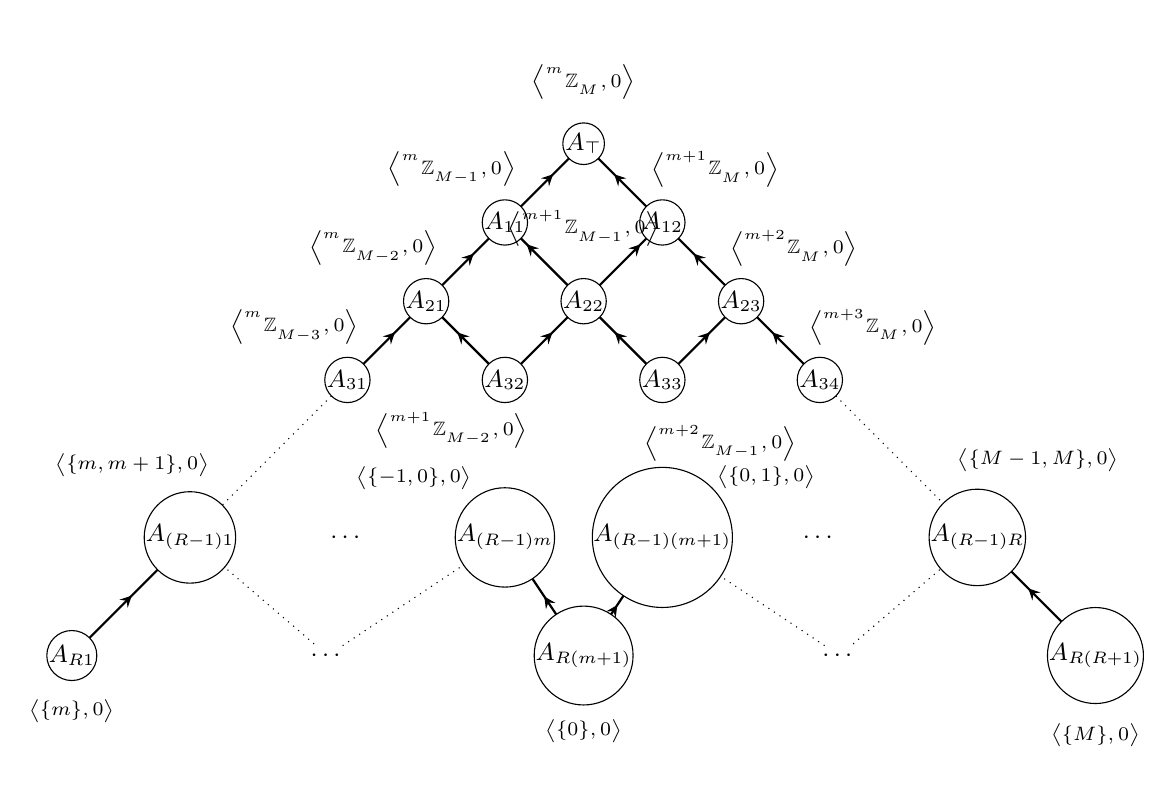
\begin{tikzpicture}[scale=0.5, every node/.style={draw, circle, inner sep=0pt, outer sep=0pt, font=\small}]
\newcommand\XRoot{12}
\newcommand\YRoot{12}
\node[label={[label distance=-5pt, font=\scriptsize]90:$\left<^{^{m}}\mathbb{Z}_{_{M}},0\right>$}] (Atop) at (\XRoot,\YRoot) {$A_\top$};
\node[label={[label distance=-5pt, font=\scriptsize]135:$\left<^{^{m}}\mathbb{Z}_{_{M-1}},0\right>$}] (A11) at (\XRoot-2,\YRoot-2) {$A_{11}$};
\node[label={[label distance=-5pt, font=\scriptsize]45:$\left<^{^{m+1}}\mathbb{Z}_{_{M}},0\right>$}] (A12) at (\XRoot+2,\YRoot-2) {$A_{12}$};
\node[label={[label distance=-5pt, font=\scriptsize]135:$\left<^{^{m}}\mathbb{Z}_{_{M-2}},0\right>$}] (A21) at (\XRoot-4,\YRoot-4) {$A_{21}$};
\node[label={[label distance=-10pt, font=\scriptsize]above:$\left<^{^{m+1}}\mathbb{Z}_{_{M-1}},0\right>$}] (A22) at (\XRoot,\YRoot-4) {$A_{22}$};
\node[label={[label distance=-5pt, font=\scriptsize]45:$\left<^{^{m+2}}\mathbb{Z}_{_{M}},0\right>$}] (A23) at (\XRoot+4,\YRoot-4) {$A_{23}$};
\node[label={[label distance=-5pt, font=\scriptsize]135:$\left<^{^{m}}\mathbb{Z}_{_{M-3}},0\right>$}] (A31) at (\XRoot-6,\YRoot-6) {$A_{31}$};
\node[label={[label distance=-10pt, font=\scriptsize]-110:$\left<^{^{m+1}}\mathbb{Z}_{_{M-2}},0\right>$}] (A32) at (\XRoot-2,\YRoot-6) {$A_{32}$};
\node[label={[label distance=-5pt, font=\scriptsize]-70:$\left<^{^{m+2}}\mathbb{Z}_{_{M-1}},0\right>$}] (A33) at (\XRoot+2,\YRoot-6) {$A_{33}$};
\node[label={[label distance=-5pt, font=\scriptsize]45:$\left<^{^{m+3}}\mathbb{Z}_{_{M}},0\right>$}] (A34) at (\XRoot+6,\YRoot-6) {$A_{34}$};
\node[label={[label distance=-10pt, font=\scriptsize]100:$\big<\{m,m+1\},0\big>$}] (All1) at (\XRoot-10,\YRoot-10) {$A_{(R-1)1}$};
\node[draw=none] at (\XRoot-6,\YRoot-10) {$\cdots$};
\node[label={[label distance=1pt, font=\scriptsize]-200:$\big<\{-1,0\},0\big>$}] (All2) at (\XRoot-2,\YRoot-10) {$A_{(R-1)m}$};
\node[label={[label distance=1pt, font=\scriptsize]20:$\big<\{0,1\},0\big>$}] (All3) at (\XRoot+2,\YRoot-10) {$A_{(R-1)(m+1)}$};
\node[draw=none] at (\XRoot+6,\YRoot-10) {$\cdots$};
\node[label={[label distance=-10pt, font=\scriptsize]80:$\big<\{M-1,M\},0\big>$}] (All4) at (\XRoot+10,\YRoot-10) {$A_{(R-1)R}$};
\node[label={[label distance=-5pt, font=\scriptsize]-90:$\big<\{m\},0\big>$}] (Al1) at (\XRoot-13,\YRoot-13) {$A_{R1}$};
\node[draw=none] (Al2) at (\XRoot-6.5,\YRoot-13) {$\cdots$};
\node[label={[label distance=-5pt, font=\scriptsize]-90:$\big<\{0\},0\big>$}] (Al3) at (\XRoot,\YRoot-13) {$A_{R(m+1)}$};
\node[draw=none] (Al4) at (\XRoot+6.5,\YRoot-13) {$\cdots$};
\node[label={[label distance=-5pt, font=\scriptsize]-90:$\big<\{M\},0\big>$}] (Al5) at (\XRoot+13,\YRoot-13) {$A_{R(R+1)}$};

\path (Atop) edge[-<-] (A11)
             edge[-<-] (A12)
      (A11)  edge[-<-] (A21)
             edge[-<-=0.3] (A22)
      (A12)  edge[-<-=0.3] (A22)
             edge[-<-] (A23)
      (A21)  edge[-<-] (A31)
             edge[-<-] (A32)
      (A22)  edge[-<-] (A32)
             edge[-<-] (A33)
      (A23)  edge[-<-] (A33)
             edge[-<-] (A34)
      (All1) edge[-<-] (Al1)
      (Al3)  edge[->-] (All2)
             edge[->-] (All3)
      (All4) edge[-<-] (Al5);
      
\path[dotted] (A31) edge (All1)
              (Al2) edge (All1)
                    edge (All2)
              (Al4) edge (All3)
                    edge (All4)
              (A34) edge (All4);
\end{tikzpicture}

\centerline{\underline{\Large{Frontal View}}}

\vspace{1cm}
\begin{itemize}
    \item $^{^{A}}\mathbb{Z}_{_{B}}=\left\{i\in\mathbb{Z}\ |\ A\leq i\leq B\right\}$
    \item $m=\mathtt{MININT}$
    \item $M=\mathtt{MAXINT}$
\end{itemize}
\begin{description}
  \item[In the Frontal View \& Lateral View (Next page):] \hfill\\
    $A_{Ri}\equiv A_{(M-m)i}\quad\text{and}\quad\hat{A}_{Ri}\equiv\hat{A}_{(M-m)i}\qquad\forall i$\\
    For every pair of indices $i, j$ (and $\top$) the elements denoted by $A_{ij}$ (and $A_\top$) and $\hat{A}_{ij}$ (and $\hat{A}_\top$) have the same interval, but probability in element $A_{ij}$ (and $A_\top$) is $0$ , wherese it is 1 for $\hat{A}_{ij}$ (and $\hat{A}_\top$).\\
    E.g: $A_{22}\equiv\left<^{^{m+1}}\mathbb{Z}_{_{M-1}},\ 0\right>$ but $\hat{A}_{22}\equiv\left<^{^{m+1}}\mathbb{Z}_{_{M-1}},\ 1\right>$
\end{description}

\newpage
\begin{tikzpicture}[x={(6mm,-3.5mm)}, y={(0mm,15mm)}, z={(14mm,0mm)}, every node/.style={inner sep=2pt}, scale=0.9, remember picture, overlay, shift={(-20mm, -86mm)}]
\newcommand\Root{8}
\newcommand\Zoffset{8}
\newcommand\InitialBlack{0.7}
\node (A1) at (\Root,\Root,0) {$A_{\top}$};
\node (A2) at (\Root-1,\Root-1,0) {$A_{11}$};
\node (A3) at (\Root+1,\Root-1,0) {$A_{12}$};
\node (A4) at (\Root-2,\Root-2,0) {$A_{21}$};
\node (A5) at (\Root,\Root-2,0) {$A_{22}$};
\node (A6) at (\Root+2,\Root-2,0) {$A_{23}$};
\node (A7) at (\Root-3,\Root-3,0) {$A_{31}$};
\node (A8) at (\Root-1,\Root-3,0) {$A_{32}$};
\node (A9) at (\Root+1,\Root-3,0) {$A_{33}$};
\node (A10) at (\Root+3,\Root-3,0) {$A_{34}$};
\node (All1) at (\Root-5,\Root-5,0) {$A_{(R-1)1}$};
\node at (\Root-3,\Root-5,0) {$\ddots$};
\node (All2) at (\Root-1,\Root-5,0) {$A_{(R-1)m}$};
\node (All3) at (\Root+1,\Root-5,0) {$A_{(R-1)(m+1)}$};
\node at (\Root+3,\Root-5,0) {$\ddots$};
\node (All4) at (\Root+5,\Root-5,0) {$A_{(R-1)R}$};
\node (Al1) at (\Root-6,\Root-6,0) {$A_{R1}$};
\node (Al2) at (\Root-3,\Root-6,0) {$\ddots$};
\node (Al3) at (\Root,\Root-6,0) {$A_{R(m+1)}$};
\node (Al4) at (\Root+3,\Root-6,0) {$\ddots$};
\node (Al5) at (\Root+6,\Root-6,0) {$A_{R(R+1)}$};

\node (B1) at (\Root,\Root,\Zoffset) {$\hat{A}_{\top}$};
\node[lightgray] (B2) at (\Root-1,\Root-1,\Zoffset) {$\hat{A}_{11}$};
\node (B3) at (\Root+1,\Root-1,\Zoffset) {$\hat{A}_{12}$};
\node[lightgray] (B4) at (\Root-2,\Root-2,\Zoffset) {$\hat{A}_{21}$};
\node[lightgray] (B5) at (\Root,\Root-2,\Zoffset) {$\hat{A}_{22}$};
\node (B6) at (\Root+2,\Root-2,\Zoffset) {$\hat{A}_{23}$};
\node[lightgray] (B7) at (\Root-3,\Root-3,\Zoffset) {$\hat{A}_{31}$};
\node[lightgray] (B8) at (\Root-1,\Root-3,\Zoffset) {$\hat{A}_{32}$};
\node[lightgray] (B9) at (\Root+1,\Root-3,\Zoffset) {$\hat{A}_{33}$};
\node (B10) at (\Root+3,\Root-3,\Zoffset) {$\hat{A}_{34}$};
\node[lightgray] (Bll1) at (\Root-5,\Root-5,\Zoffset) {$\hat{A}_{(R-1)1}$};
\node[lightgray] (Bll2) at (\Root-1,\Root-5,\Zoffset) {$\hat{A}_{(R-1)m}$};
\node[lightgray] (Bll3) at (\Root+1,\Root-5,\Zoffset) {$\hat{A}_{(R-1)(m+1)}$};
\node (Bll4) at (\Root+5,\Root-5,\Zoffset) {$\hat{A}_{(R-1)R}$};
\node[lightgray] (Bl1) at (\Root-6,\Root-6,\Zoffset) {$\hat{A}_{R1}$};
\node[lightgray] (Bl2) at (\Root-3,\Root-6,\Zoffset) {$\ddots$};
\node[lightgray] (Bl3) at (\Root,\Root-6,\Zoffset) {$\hat{A}_{R(m+1)}$};
\node[lightgray] (Bl4) at (\Root+3,\Root-6,\Zoffset) {$\ddots$};
\node (Bl5) at (\Root+6,\Root-6,\Zoffset) {$\hat{A}_{R(R+1)}$};
\node (Bottom) at (\Root,\Root-8,\Zoffset) {$A_{\bot}=\langle\{\},1\rangle$};

\path[dashed] (A1)   edge[-<-] (B1)
              (A3)   edge[-<-] (B3)
              (A6)   edge[-<-] (B6)
              (A10)  edge[-<-] (B10)
              (All4) edge[-<-] (Bll4)
              (Al5)  edge[-<-] (Bl5);

\draw[dashed] (A2) -- (\Root-1,\Root-1,\InitialBlack) (A4) -- (\Root-2,\Root-2,\InitialBlack) (A5) -- (\Root,\Root-2,\InitialBlack) (A7) -- (\Root-3,\Root-3,\InitialBlack) (A8) -- (\Root-1,\Root-3,\InitialBlack) (A9) -- (\Root+1,\Root-3,\InitialBlack) (All1) -- (\Root-5,\Root-5,\InitialBlack*5) (All2) -- (\Root-1,\Root-5,\InitialBlack*3) (All3) -- (\Root+1,\Root-5,\InitialBlack*2) (Al1) -- (\Root-6,\Root-6,\InitialBlack*1.2) (Al3) -- (\Root,\Root-6,\InitialBlack*1.2);

\draw[lightgray, dashed] (\Root-1,\Root-1,\InitialBlack) -- (B2) (\Root-2,\Root-2,\InitialBlack) -- (B4) (\Root,\Root-2,\InitialBlack) -- (B5) (\Root-3,\Root-3,\InitialBlack) -- (B7) (\Root-1,\Root-3,\InitialBlack) -- (B8) (\Root+1,\Root-3,\InitialBlack) -- (\Root+1,\Root-3,\Zoffset) (\Root-5,\Root-5,\InitialBlack*5) -- (Bll1) (\Root-1,\Root-5,\InitialBlack*3) -- (Bll2) (\Root+1,\Root-5,\InitialBlack*2) -- (Bll3) (\Root-6,\Root-6,\InitialBlack*1.2) -- (Bl1) (\Root,\Root-6,\InitialBlack*1.2) -- (Bl3);

\draw (A1) edge[-<-] (A2) (A2) edge[-<-] (A4) (A4) edge[-<-] (A7) (A1) edge[-<-] (A3) (A3) edge[-<-] (A6) (A6) edge[-<-] (A10);

\draw (A2) edge[-<-] (A5) (A3) edge[-<-] (A5) (A4) edge[-<-] (A8) (A5) edge[-<-] (A8) (A5) edge[-<-] (A9) (A6) edge[-<-] (A9) (All1) edge[-<-] (Al1) (All4) edge[-<-] (Al5) (All2) edge[-<-] (Al3) (All3) edge[-<-] (Al3) (Bl5) edge[-<-] (Bottom) (Bottom) -- (\Root+6,\Root-6,\Zoffset*0.679) (Bottom) -- (\Root+5.75,\Root-6.05,\Zoffset*0.64);

\draw[dotted] (A7) -- (All1) -- (Al2) (A10) -- (All4) -- (Al4) (All2) -- (Al2) (All3) -- (Al4) (B10) -- (Bll4) (Bl2) -- (Bottom) -- (Bl4);

\draw (B1) edge[-<-=0.3] (B3) (B3) edge[-<-=0.4] (B6) (B6) edge[-<-=0.4] (B10) (Bll4) edge[-<-=0.4] (Bl5);

\draw[lightgray, dotted] (B7) edge (Bll1) (Bll1) edge (Bl2) (Bll2) edge (Bl2) (Bll3) edge (Bl4) (Bll4) edge (Bl4);

\draw[lightgray] (B1) edge[-<-] (B2) (B2) edge[-<-=0.4] (B4) (B2) edge[-<-=0.6] (B5) (B3) edge[-<-] (B5) (B4) edge[-<-=0.4] (B7) (B4) edge[-<-] (B8) (B5) edge[-<-=0.4] (B8) (B5) edge[-<-=0.7] (B9) (B6) edge[-<-=0.7] (B9) (Bll1) edge[-<-] (Bl1) (Bll2) edge[-<-=0.6] (Bl3) (Bll3) edge[-<-=0.6] (Bl3) (Bl3) edge[-<-] (\Root+6,\Root-6,\Zoffset*0.679) (\Root+5.75,\Root-6.05,\Zoffset*0.64) edge[->-=0.7] (Bl1);
\end{tikzpicture}
\\\\\\\\\\\\\\\\\\\\\\\\\\\\\\\\\\
\centerline{\underline{\Large{Lateral View (Skewed)}}}
\begin{tikzpicture}[remember picture, overlay, shift={(0mm, -86mm)}]
\newcommand\XRoot{8}
\newcommand\YRoot{8}
\node (Top) at (\XRoot,\YRoot) {$\hat{A}_\top$};
\node (A12) at (\XRoot-1,\YRoot-1) {$\hat{A}_{12}$};
\node (A11) at (\XRoot+1,\YRoot-1) {$\hat{A}_{11}$};
\node (A23) at (\XRoot-2,\YRoot-2) {$\hat{A}_{23}$};
\node (A22) at (\XRoot,\YRoot-2) {$\hat{A}_{22}$};
\node (A21) at (\XRoot+2,\YRoot-2) {$\hat{A}_{21}$};
\node (A34) at (\XRoot-3,\YRoot-3) {$\hat{A}_{34}$};
\node (A33) at (\XRoot-1,\YRoot-3) {$\hat{A}_{33}$};
\node (A32) at (\XRoot+1,\YRoot-3) {$\hat{A}_{32}$};
\node (A31) at (\XRoot+3,\YRoot-3) {$\hat{A}_{31}$};
\node (All1) at (\XRoot-5,\YRoot-5) {$\hat{A}_{(R-1)R}$};
\node (All2) at (\XRoot-3,\YRoot-5) {$\cdots$};
\node (All3) at (\XRoot-1,\YRoot-5) {$\hat{A}_{(R-1)(m+1)}$};
\node (All4) at (\XRoot+1,\YRoot-5) {$\hat{A}_{(R-1)m}$};
\node (All5) at (\XRoot+3,\YRoot-5) {$\cdots$};
\node (All6) at (\XRoot+5,\YRoot-5) {$\hat{A}_{(R-1)1}$};
\node (Al1) at (\XRoot-6,\YRoot-6) {$\hat{A}_{R(R+1)}$};
\node (Al2) at (\XRoot-3,\YRoot-6) {$\cdots$};
\node (Al3) at (\XRoot,\YRoot-6) {$\hat{A}_{R(m+1)}$};
\node (Al4) at (\XRoot+3,\YRoot-6) {$\cdots$};
\node (Al5) at (\XRoot+6,\YRoot-6) {$\hat{A}_{R1}$};
\node (Bottom) at (\XRoot,\YRoot-8) {$A_\bot$};

\path (Bottom) edge[->-] (Al1)
               edge[->-] (Al3)
               edge[->-] (Al5);

\path (Top) edge[-<-] (A12) (Top) edge[-<-] (A11) (A12) edge[-<-] (A23) (A12) edge[-<-] (A22) (A11) edge[-<-] (A22) (A11) edge[-<-] (A21) (A23) edge[-<-] (A34) (A23) edge[-<-] (A33) (A22) edge[-<-] (A33) (A22) edge[-<-] (A32) (A21) edge[-<-] (A32) (A21) edge[-<-] (A31) (All1) edge[-<-] (Al1) (All3) edge[-<-] (Al3) (All4) edge[-<-] (Al3) (All6) edge[-<-] (Al5);

\draw[dotted] (Al2) -- (Bottom) -- (Al4) (A34) -- (All1) (A31) -- (All6) (All1) -- (Al2) -- (All3) (All4) -- (Al4) -- (All6);
\end{tikzpicture}
\\\\\\\\\\\\\\\\\\\\\\\\\\\\\\
\centerline{\underline{\Large{Rear View}}}








\section{\\Proof of $\sqsubseteq_M$ being a partial order}
\label{app:interval_partial}

We prove that $\sqsubseteq_M$ is a partial order relation as follows.

\begin{description}
\item[Reflexivity :] \hfill \\
	It's trivial to show that $\langle[a,b],p_{ab}\rangle\sqsubseteq_M\langle[a,b],p_{ab}\rangle$. It follows directly from the Definition~\ref{abstract_order}.
\item[Transitivity :] \hfill \\
	$\langle[a,b],p_{ab}\rangle\sqsubseteq_M\langle[c,d],p_{cd}\rangle\qquad\qquad\mathrm{and}\qquad\qquad\langle[c,d],p_{cd}\rangle\sqsubseteq_M\langle[e,f],p_{ef}\rangle\hfill$ (Given)	
\begin{alignat}{2}
    [a,b]\sqsubseteq_{int}[c,d] &\qquad\land\qquad[c,d]\sqsubseteq_{int}[e,f]\label{eq:po1}\\
	p.m.f\Big(\langle[a,b],p_{ab}\rangle\Big)\geq\ p.m.f\Big(\langle[c,d],p_{cd}\rangle\Big) &\qquad\land\qquad p.m.f\Big(\langle[c,d],p_{cd}\rangle\Big)\geq\ p.m.f\Big(\langle[e,f],p_{ef}\rangle\Big)\label{eq:po2}
\end{alignat}
	
\noindent From Equation~\ref{eq:po1} we get $[a,b]\sqsubseteq_{int}[e,f]$ and from Equation~\ref{eq:po2} we get $p.m.f\Big(\langle[a,b],p_{ab}\rangle\Big)\geq\ p.m.f\Big(\langle[e,f],p_{ef}\rangle\Big)$.
	
	$\therefore\langle[a,b],p_{ab}\rangle\sqsubseteq_M\langle[e,f],p_{ef}\rangle$
\item[Anti-Symmetricity :] \hfill \\
	$\langle[a,b],p_{ab}\rangle\sqsubseteq_M\langle[c,d],p_{cd}\rangle\qquad\qquad\mathrm{and}\qquad\qquad\langle[c,d],p_{cd}\rangle\sqsubseteq_M\langle[a,b],p_{ab}\rangle\hfill$ (Given)
\begin{alignat}{2}
    [a,b]\sqsubseteq_{int}[c,d]\implies (c\leq a)\land (b\leq d)&\qquad\qquad\Big[\mathrm{From\ Definition}~\ref{interval_def}\Big]\label{eq:po3}\\
	[c,d]\sqsubseteq_{int}[a,b]\implies (a\leq c)\land (d\leq b)&\qquad\qquad\Big[\mathrm{From\ Definition}~\ref{interval_def}\Big]\label{eq:po4}\\
	p.m.f\Big(\langle[a,b],p_{ab}\rangle\Big)\geq p.m.f\Big(\langle[c,d],p_{cd}\rangle\Big)&\label{eq:po5}\\
	p.m.f\Big(\langle[c,d],p_{cd}\rangle\Big)\geq p.m.f\Big(\langle[a,b],p_{ab}\rangle\Big)&\label{eq:po6}
\end{alignat}

\noindent Combining Equation~\ref{eq:po3} and Equation~\ref{eq:po4} we get,\\
	$(c\leq a)\land (a\leq c)\implies a=c$ and\\
	$(b\leq d)\land (d\leq b)\implies b=d$\\
	$\therefore a=c,\ b=d$
	
\noindent From Equation~\ref{eq:po5} and Equation~\ref{eq:po6} we get,\\
	$p.m.f\Big(\langle[a,b],p_{ab}\rangle\Big)=p.m.f\Big(\langle[c,d],p_{cd}\rangle\Big)$\\
	$\Rightarrow \displaystyle\frac{p_{ab}}{b-a+1}=\frac{p_{cd}}{d-c+1}\hfill\Big[\mathrm{From\ Definition}~\ref{pmf}\Big]$\\
	$\Rightarrow p_{ab}=p_{cd}\hfill\Big[\because a=c,\ b=d\quad\mathrm{and}\quad b-a+1\neq0\Big]$
	
	$\therefore\langle[a,b],p_{ab}\rangle=\langle[c,d],p_{cd}\rangle$
\end{description}








\section{\\Proof of correctness of the $l.u.b \displaystyle\bigsqcup_M$ and $g.l.b \displaystyle\bigsqcap^M$ operators in $M$}
\label{app:interval_ub}

\usetikzlibrary{arrows}
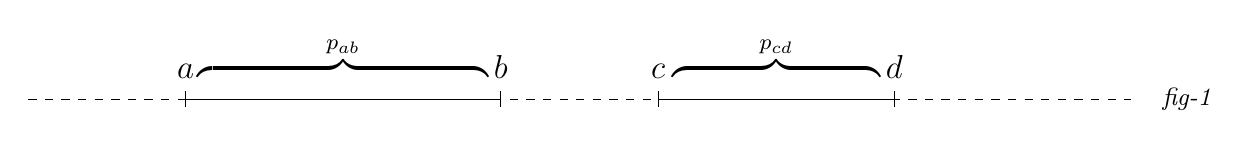
\begin{tikzpicture}[font=\large]
\draw [dashed] (0,0) -- (14,0);
\foreach \x in {2,6,8,11}
\draw [shift={(\x,0)},color=black] (0,3pt) -- (0,-3pt);
\draw (2,0) -- (6,0);
\draw (8,0) -- (11,0);
\draw (2,0) node[above=4pt]{$a$};
\draw (6,0) node[above=4pt]{$b$};
\draw (8,0) node[above=4pt]{$c$};
\draw (11,0) node[above=4pt]{$d$};
\draw (4,0) node[above=4pt]{$\overbrace{\hspace{105pt}}^{p_{ab}}$};
\draw (9.5,0) node[above=4pt]{$\overbrace{\hspace{75pt}}^{p_{cd}}$};
\draw (14,0) node[right=8pt]{\small{\textit{fig-1}}};
\end{tikzpicture}

\noindent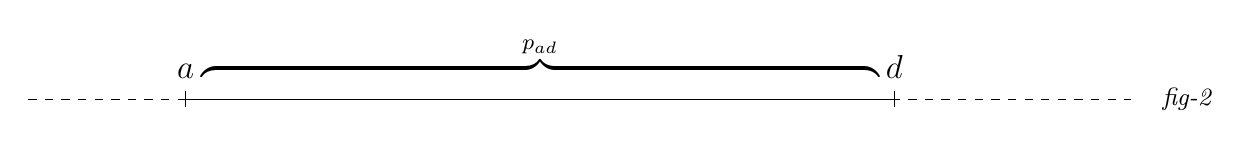
\begin{tikzpicture}[font=\large]
\draw [dashed] (0,0) -- (14,0);
\foreach \x in {2,11}
\draw [shift={(\x,0)},color=black] (0,3pt) -- (0,-3pt);
\draw (2,0) -- (11,0);
\draw (2,0) node[above=4pt]{$a$};
\draw (11,0) node[above=4pt]{$d$};
\draw (6.5,0) node[above=4pt]{$\overbrace{\hspace{245pt}}^{p_{ad}}$};
\draw (14,0) node[right=8pt]{\small{\textit{fig-2}}};
\end{tikzpicture}

\noindent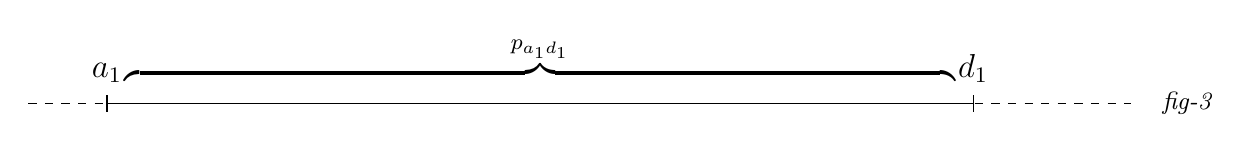
\begin{tikzpicture}[font=\large]
\draw [dashed] (0,0) -- (14,0);
\foreach \x in {1,12}
\draw [shift={(\x,0)},color=black] (0,3pt) -- (0,-3pt);
\draw (1,0) -- (12,0);
\draw (1,0) node[above=4pt]{$a_1$};
\draw (12,0) node[above=4pt]{$d_1$};
\draw (6.5,0) node[above=4pt]{$\overbrace{\hspace{300pt}}^{p_{a_1d_1}}$};
\draw (14,0) node[right=8pt]{\small{\textit{fig-3}}};
\end{tikzpicture}\\

\noindent For the two elements $\langle[a,b],p_{ab}\rangle$ and $\langle[c,d],p_{cd}\rangle$ (in \small{\textit{fig-1}}) suppose the $l.u.b$ is $\langle[x,y],p_{xy}\rangle$, i.e
\[ \displaystyle\langle[a,b],p_{ab}\rangle\ \bigsqcup_M\ \langle[c,d],p_{cd}\rangle=\langle[x,y],p_{xy}\rangle \]
From Equation~\ref{eq:lub_M} we get,
\[ x=\mathbf{min}(a,c)=a\qquad y=\mathbf{max}(b,d)=d\qquad\displaystyle p_{xy}=(d-a+1)\ \cdot\ \mathbf{min}\left(p.m.f\Big(\big<[a,\ b],\ p_{ab}\big>\Big),\ p.m.f\Big(\big<[c,\ d],\ p_{cd}\big>\Big),\ \frac{1}{d-a+1}\right) \]

$\therefore\langle[a,d],p_{ad}\rangle$ (in \small{\textit{fig-2}}) is the $l.u.b$ of the elements in \small{\textit{fig-1}} with $p_{ad}=p_{xy}$. Now we show, all upper bounds of $\langle[a,b],p_{ab}\rangle$ and $\langle[c,d],p_{cd}\rangle$ come higher in the order than $\langle[a,d],p_{ad}\rangle$.

It's trivial to show that for any tuple of the form $\langle[a,d],p'_{ad}\rangle$, where $p'_{ad}\leq p_{ad}\footnote{If $p'_{ad}>p_{ad}$, then $\langle[a,d],p'_{ad}\rangle$ is \textbf{NOT} an upper bound of both $\langle[a,b],p_{ab}\rangle$ and $\langle[c,d],p_{cd}\rangle$}$, $\langle[a,d],p_{ad}\rangle\sqsubseteq_M\langle[a,d],p'_{ad}\rangle$ (By Definition~\ref{abstract_order}). So, $\langle[a,d],p_{ad}\rangle$ remains the $l.u.b$.

Now, the other form of tuple i.e $\langle[a_1,d_1],p_{a_1d_1}\rangle$ (in \small{\textit{fig-3}}), where $[a,d]\sqsubseteq_{int}[a_1,d_1]$, will be an upper bound of $\langle[a,b],p_{ab}\rangle$ and $\langle[c,d],p_{cd}\rangle$ if\\
$\langle[a,b],p_{ab}\rangle\sqsubseteq_M\langle[a_1,d_1],p_{a_1d_1}\rangle\qquad\bigwedge\qquad\langle[c,d],p_{cd}\rangle\sqsubseteq_M\langle[a_1,d_1],p_{a_1d_1}\rangle$\\
$\Rightarrow p.m.f\Big(\langle[a_1,d_1],p_{a_1d_1}\rangle\Big)\leq p.m.f\Big(\langle[a,b],p_{ab}\rangle\Big)\ \bigwedge\ p.m.f\Big(\langle[a_1,d_1],p_{a_1d_1}\rangle\Big)\leq p.m.f\Big(\langle[c,d],p_{cd}\rangle\Big)\hfill\Big[\because \text{we\ know\ }[a,d]\sqsubseteq_{int}[a_1,d_1]\Big]$\\
$\Rightarrow p_{a_1d_1}\leq(d_1-a_1+1)\cdot p.m.f\Big(\langle[a,b],p_{ab}\rangle\Big)\ \bigwedge\ p_{a_1d_1}\leq(d_1-a_1+1)\cdot p.m.f\Big(\langle[c,d],p_{cd}\rangle\Big)\hfill\Big[\text{From\ Definition}~\ref{pmf}\Big]$\\
$\Rightarrow p_{a_1d_1}\leq\mathbf{min}\left((d_1-a_1+1)\cdot p.m.f\Big(\langle[a,b],p_{ab}\rangle\Big),\ (d_1-a_1+1)\cdot p.m.f\Big(\langle[c,d],p_{cd}\rangle\Big),\ 1\right)\hfill\Big[\because p_{a_1d_1}\leq1\Big]$\\
$\Rightarrow\displaystyle p_{a_1d_1}\leq(d_1-a_1+1)\ \cdot\ \mathbf{min}\left(p.m.f\Big(\big<[a,\ b],\ p_{ab}\big>\Big),\ p.m.f\Big(\big<[c,\ d],\ p_{cd}\big>\Big),\ \frac{1}{d_1-a_1+1}\right)$

\noindent We need to prove that, $p.m.f\Big(\big<[a,\ d],\ p_{ad}\big>\Big)\geq p.m.f\Big(\big<[a_1,\ d_1],\ p_{a_1d_1}\big>\Big)$, in order to prove that $\big<[a,\ d],\ p_{ad}\big>$ still remains the $l.u.b$.

\noindent Without any loss of generality, we assume that
\begin{alignat}{2}
p.m.f\Big(\langle[a,b],p_{ab}\rangle\Big)\leq p.m.f\Big(\langle[c,d],p_{cd}\rangle\Big)\label{eq:ub1}\\
\frac{1}{d_1-a_1+1}<\frac{1}{d-a+1}\label{eq:ub2}
\end{alignat}
\begin{equation*}
 \left.\begin{aligned}
        p_{ad}&=(d-a+1)\ \cdot\ \mathbf{min}\left(p.m.f\Big(\langle[a,b],p_{ab}\rangle\Big),\ p.m.f\Big(\langle[c,d],p_{cd}\rangle\Big),\ \frac{1}{d-a+1}\right)\\
        &=(d-a+1)\ \cdot\ \mathbf{min}\left(p.m.f\Big(\langle[a,b],p_{ab}\rangle\Big),\ \frac{1}{d-a+1}\right)\qquad\qquad\qquad[\text{From Equation}~\ref{eq:ub1}]\\
        p_{a_1d_1}&=(d_1-a_1+1)\ \cdot\ \mathbf{min}\left(p.m.f\Big(\langle[a,b],p_{ab}\rangle\Big),\ p.m.f\Big(\langle[c,d],p_{cd}\rangle\Big),\ \frac{1}{d_1-a_1+1}\right)\\
        &=(d_1-a_1+1)\ \cdot\ \mathbf{min}\left(p.m.f\Big(\langle[a,b],p_{ab}\rangle\Big),\ \frac{1}{d_1-a_1+1}\right)\qquad\qquad[\text{From Equation}~\ref{eq:ub1}]
       \end{aligned}\qquad
 \right\}\hfill\text{(Given)}
\end{equation*}

In view of Equation~\ref{eq:ub2} there are three cases to consider now.

\begin{description}
	\item[Case 1 : $\qquad\displaystyle p.m.f\Big(\langle\lbrack a,b\rbrack,p_{ab}\rangle\Big)\leq\frac{1}{d_1-a_1+1}$] \hfill
	\[ \therefore \displaystyle p.m.f\Big(\langle[a,b],p_{ab}\rangle\Big)<\frac{1}{d-a+1}\hfill\text{[From Equation~\ref{eq:ub2}]}\]
	\[ \therefore p_{ad}=(d-a+1)\ \cdot\ p.m.f\Big(\langle[a,b],p_{ab}\rangle\Big),\qquad p_{a_1d_1}=(d_1-a_1+1)\ \cdot\ p.m.f\Big(\langle[a,b],p_{ab}\rangle\Big) \]
	\[ \therefore p.m.f\Big(\langle[a,d],p_{ad}\rangle\Big)=p.m.f\Big(\langle[a_1,d_1],p_{a_1d_1}\rangle\Big) \]
	\item[Case 2 : $\qquad\displaystyle \frac{1}{d_1-a_1+1}<p.m.f\Big(\langle\lbrack a,b\rbrack,p_{ab}\rangle\Big)<\frac{1}{d-a+1}$] \hfill
	\[ \therefore p_{ad}=(d-a+1)\ \cdot\ p.m.f\Big(\langle[a,b],p_{ab}\rangle\Big),\qquad p_{a_1d_1}=1 \]
	\[ \therefore p.m.f\Big(\langle[a,d],p_{ad}\rangle\Big)=p.m.f\Big(\langle[a,b],p_{ab}\rangle\Big),\qquad p.m.f\Big(\langle[a_1,d_1],p_{a_1d_1}\rangle\Big)=\frac{1}{d_1-a_1+1} \]
	\[ \therefore p.m.f\Big(\langle[a,d],p_{ad}\rangle\Big)>p.m.f\Big(\langle[a_1,d_1],p_{a_1d_1}\rangle\Big) \]
	\item[Case 3 : $\qquad\displaystyle \frac{1}{d-a+1}\leq p.m.f\Big(\langle\lbrack a,b\rbrack,p_{ab}\rangle\Big)$] \hfill
	\[ \therefore \displaystyle p.m.f\Big(\langle[a,b],p_{ab}\rangle\Big)>\frac{1}{d_1-a_1+1}\hfill\text{[From Equation~\ref{eq:ub2}]} \]
	\[ \therefore p_{ad}=1,\qquad p_{a_1d_1}=1 \]
	\[ \therefore p.m.f\Big(\langle[a,d],p_{ad}\rangle\Big)=\ p.m.f\Big(\langle[a_1,d_1],p_{a_1d_1}\rangle\Big) \]
\end{description}

\noindent In all the above three cases $p.m.f\Big(\langle[a,d],p_{ad}\rangle\Big)\geq p.m.f\Big(\langle[a_1,d_1],p_{a_1d_1}\rangle\Big)$. Hence $\langle[a,d],p_{ad}\rangle$ is the least upper bound.

\noindent Analogous arguments can be applied to show the soundness of the greatest lower bound, $\displaystyle\bigsqcap^M$ definition.






\section{\\Proof of monotonicity of Galois connection $(\alpha,\gamma)$}
\label{app:monotonicity}

From Definition~\ref{gamma}, we have,

\begin{tabular}{@{\hspace{2mm}}rcl}
  $\GAMMA$$\Big(\big\langle[\ ],\ 1\big\rangle\Big)$ & = & $\Big\langle\big\{\ \big\},\ 1\Big\rangle=\perp_L$\\
  $\GAMMA$$\Big(\big\langle[a,\ b],\ p_{ab}\big\rangle\Big)$ & = & $\bigg\langle\bigg\{i\in\mathbb{Z}\ :\ a\leq i\leq b\bigg\},\ p.m.f\Big(\langle[a,b],p_{ab}\rangle\Big)\bigg\rangle$
\end{tabular}

\noindent Let, $\langle[a,b],p_{ab}\rangle$ and $\langle[c,d],p_{cd}\rangle$ be two elements in $M$, with $\langle[a,b],p_{ab}\rangle\sqsubseteq_M\langle[c,d],p_{cd}\rangle$\footnote{If $\quad\perp_M\sqsubseteq_M\langle[a,b],p_{ab}\rangle$, we trivially have $\quad$$\GAMMA$$\Big(\perp_M\Big)\sqsubseteq_L\ $$\GAMMA$$\Big(\langle[a,b],p_{ab}\rangle\Big)\quad$[$\ \because$$\GAMMA$$\Big(\perp_M\Big)=\perp_L$ is the least element in $\mathcal{L}$]}. We show that $\GAMMA$$\Big(\langle[a,b],p_{ab}\rangle\Big)\sqsubseteq_L\ $$\GAMMA$$\Big(\langle[c,d],p_{cd}\rangle\Big)$

\noindent$\because\langle[a,b],p_{ab}\rangle\sqsubseteq_M\langle[c,d],p_{cd}\rangle$, from the Definition~\ref{abstract_order} we have
\begin{flalign}
  &[a,b]\sqsubseteq_{int}[c,d]\qquad\qquad\text{and}\nonumber&&\\
  &p.m.f\big(\langle[a,b],p_{ab}\rangle\big)\geq p.m.f\big(\langle[c,d],p_{cd}\rangle\big)\label{eq:monotone1}&&
\end{flalign}
\begin{flalign}
  &\quad[a,b]\sqsubseteq_{int}[c,d]&\nonumber\\
  \Rightarrow &\quad c\leq a\bigwedge b\leq d&[\text{From Definition}~\ref{interval_def}]\nonumber\\
  \Rightarrow &\quad\{i\in\mathbb{Z}\ |\ a\leq i\leq b\}\subseteq\{i\in\mathbb{Z}\ |\ c\leq i\leq d\}\label{eq:monotone2}&
\end{flalign}

\noindent From Equation~\ref{eq:monotone1} and Equation~\ref{eq:monotone2} we get, $\qquad$$\GAMMA$$\Big(\langle[a,b],p_{ab}\rangle\Big)\sqsubseteq_L\ $$\GAMMA$$\Big(\langle[c,d],p_{cd}\rangle\Big)$\hfill[Using Definition~\ref{concrete_order}]

\noindent This completes the proof that $\GAMMA$ is monotonic.

\noindent\rule{14cm}{0.1pt}

\noindent From Definition~\ref{alpha}, we have,
\begin{align*}
\ALPHA\big(\langle S,p\rangle\big)= 
  \begin{cases} 
    \big\langle[\ ],\ 1\big\rangle=\perp_M        &        \langle S,p\rangle=\langle\phi,1\rangle=\perp_L\\
    \bigg\langle\Big[\mathcal{V}_m\Big(\langle S,p\rangle\Big),\ \mathcal{V}_M\Big(\langle S,p\rangle\Big)\Big],\ \mathbf{min}\bigg(1,\ p\cdot\Big(\mathcal{V}_M\Big(\langle S,p\rangle\Big)-\mathcal{V}_m\Big(\langle S,p\rangle\Big)+1\Big)\bigg)\bigg\rangle        &        \text{otherwise}
  \end{cases} 
\end{align*}

\noindent Now, suppose $\langle S_1,p_1\rangle$ and $\langle S_2,p_2\rangle$ are two elements in $L$, with $\langle S_1,p_1\rangle\sqsubseteq_L\langle S_2,p_2\rangle$ and $S_1\neq\phi$\footnote{If $\quad S_1=\phi$, we have $\langle S_1,p_1\rangle=\perp_L\sqsubseteq_L\langle S_2,p_2\rangle\ \Rightarrow\ $$\ALPHA$$\Big(\perp_L\Big)\sqsubseteq_M\ $$\ALPHA$$\Big(\langle S_2,p_2\rangle\Big),\quad[\ \because\ $$\ALPHA$$\Big(\perp_L\Big)=\langle[],1\rangle=\perp_M,\ $ the least element of $\mathcal{M}]$.}. We show that $\ALPHA$$\Big(\langle S_1,p_1\rangle\Big)\sqsubseteq_M\ $$\ALPHA$$\Big(\langle S_2,p_2\rangle\Big)$

\noindent $\because\langle S_1,p_1\rangle\sqsubseteq_L\langle S_2,p_2\rangle$, from the Definition~\ref{concrete_order}, we have,
\begin{flalign}
  &S_1\subseteq S_2\label{eq:monotone3}&&\\
  &p_1\geq p_2\label{eq:monotone4}&&
\end{flalign}

\noindent$\ALPHA$$\big(\langle S_1,p_1\rangle\big) = \bigg\langle\Big[\mathcal{V}_m\Big(\langle S_1,p_1\rangle\Big),\ \mathcal{V}_M\Big(\langle S_1,p_1\rangle\Big)\Big],\ \mathbf{min}\bigg(1,\ p_1\cdot\Big(\mathcal{V}_M\Big(\langle S_1,p_1\rangle\Big)-\mathcal{V}_m\Big(\langle S_1,p_1\rangle\Big)+1\Big)\bigg)\bigg\rangle\qquad$ and

\noindent$\ALPHA$$\big(\langle S_2,p_2\rangle\big) = \bigg\langle\Big[\mathcal{V}_m\Big(\langle S_2,p_2\rangle\Big),\ \mathcal{V}_M\Big(\langle S_2,p_2\rangle\Big)\Big],\ \mathbf{min}\bigg(1,\ p_2\cdot\Big(\mathcal{V}_M\Big(\langle S_2,p_2\rangle\Big)-\mathcal{V}_m\Big(\langle S_2,p_2\rangle\Big)+1\Big)\bigg)\bigg\rangle$\\

\noindent From Equation~\ref{eq:monotone3}, we get,
\begin{flalign}
&\quad\mathcal{V}_m\Big(\langle S_2,p_2\rangle\Big)\leq\mathcal{V}_m\Big(\langle S_1,p_1\rangle\Big)\ \bigwedge\ \mathcal{V}_M\Big(\langle S_1,p_1\rangle\Big)\leq\mathcal{V}_M\Big(\langle S_2,p_2\rangle\Big)&&\nonumber\\
\Rightarrow&\quad\Big[\mathcal{V}_m\Big(\langle S_1,p_1\rangle\Big),\ \mathcal{V}_M\Big(\langle S_1,p_1\rangle\Big)\Big]\ \sqsubseteq_{int}\ \Big[\mathcal{V}_m\Big(\langle S_2,p_2\rangle\Big),\ \mathcal{V}_M\Big(\langle S_2,p_2\rangle\Big)\Big]\qquad\qquad\text{[Using Definition~\ref{interval_def}]}&&\label{eq:monotone5}
\end{flalign}

\noindent From Equation~\ref{eq:monotone5}, we get,
  \begin{flalign}
    &\quad\mathcal{V}_M\Big(\langle S_1,p_1\rangle\Big)-\mathcal{V}_m\Big(\langle S_1,p_1\rangle\Big)+1\leq\mathcal{V}_M\Big(\langle S_2,p_2\rangle\Big)-\mathcal{V}_m\Big(\langle S_2,p_2\rangle\Big)+1&&\nonumber\\
    \Rightarrow&\quad\displaystyle\frac{1}{\mathcal{V}_M\Big(\langle S_1,p_1\rangle\Big)-\mathcal{V}_m\Big(\langle S_1,p_1\rangle\Big)+1}\geq\displaystyle\frac{1}{\mathcal{V}_M\Big(\langle S_2,p_2\rangle\Big)-\mathcal{V}_m\Big(\langle S_2,p_2\rangle\Big)+1}&&\label{eq:monotone6}
  \end{flalign}
  
\noindent$p.m.f\Big($$\ALPHA$$\big(\langle S_i,p_i\rangle\big)\Big) = \mathbf{min}\left(p_i,\displaystyle\frac{1}{\mathcal{V}_M\Big(\langle S_i,p_i\rangle\Big)-\mathcal{V}_m\Big(\langle S_i,p_i\rangle\Big)+1}\right)\qquad\forall i\in\{1,2\}$

\noindent Now, depending upon the values of $\quad p.m.f\Big($$\ALPHA$$\big(\langle S_1,p_1\rangle\big)\Big)\quad$ and $\quad p.m.f\Big($$\ALPHA$$\big(\langle S_2,p_2\rangle\big)\Big),\quad$ we have 4 different cases to consider.

\begin{description}
  \item[Case 1 :] $p.m.f\Big($$\ALPHA$$\big(\langle S_1,p_1\rangle\big)\Big)=p_1\qquad$ and $\qquad p.m.f\Big($$\ALPHA$$\big(\langle S_2,p_2\rangle\big)\Big)=p_2$ \hfill \\
    From Equation~\ref{eq:monotone4}, it's obvious that $\qquad p.m.f\Big($$\ALPHA$$\big(\langle S_1,p_1\rangle\big)\Big)\geq p.m.f\Big($$\ALPHA$$\big(\langle S_2,p_2\rangle\big)\Big)$
  
  \item[Case 2 :] $p.m.f\Big($$\ALPHA$$\big(\langle S_1,p_1\rangle\big)\Big)=p_1\qquad$ and $\qquad p.m.f\Big($$\ALPHA$$\big(\langle S_2,p_2\rangle\big)\Big)=\displaystyle\frac{1}{\mathcal{V}_M\Big(\langle S_2,p_2\rangle\Big)-\mathcal{V}_m\Big(\langle S_2,p_2\rangle\Big)+1}$ \hfill \\
    
    $\because\ p.m.f\Big($$\ALPHA$$\big(\langle S_2,p_2\rangle\big)\Big)=\displaystyle\frac{1}{\mathcal{V}_M\Big(\langle S_2,p_2\rangle\Big)-\mathcal{V}_m\Big(\langle S_2,p_2\rangle\Big)+1}$
    \begin{flalign*}
      \Rightarrow&\quad p_2\geq\frac{1}{\mathcal{V}_M\Big(\langle S_2,p_2\rangle\Big)-\mathcal{V}_m\Big(\langle S_2,p_2\rangle\Big)+1}&&\\
      \Rightarrow&\quad p_1\geq\frac{1}{\mathcal{V}_M\Big(\langle S_2,p_2\rangle\Big)-\mathcal{V}_m\Big(\langle S_2,p_2\rangle\Big)+1} & \text{[From Equation~\ref{eq:monotone4}]} &
    \end{flalign*}
  $\therefore\ p.m.f\Big($$\ALPHA$$\big(\langle S_1,p_1\rangle\big)\Big)\geq p.m.f\Big($$\ALPHA$$\big(\langle S_2,p_2\rangle\big)\Big)$
  
  \item[Case 3 :] $p.m.f\Big($$\ALPHA$$\big(\langle S_1,p_1\rangle\big)\Big)=\displaystyle\frac{1}{\mathcal{V}_M\Big(\langle S_1,p_1\rangle\Big)-\mathcal{V}_m\Big(\langle S_1,p_1\rangle\Big)+1}\qquad$ and $\qquad p.m.f\Big($$\ALPHA$$\big(\langle S_2,p_2\rangle\big)\Big)=p_2$ \hfill \\
  
  $\because\ p.m.f\Big($$\ALPHA$$\big(\langle S_2,p_2\rangle\big)\Big)=p_2$
    \begin{flalign*}
      \Rightarrow&\quad\frac{1}{\mathcal{V}_M\Big(\langle S_2,p_2\rangle\Big)-\mathcal{V}_m\Big(\langle S_2,p_2\rangle\Big)+1}\geq p_2&&\\
      \Rightarrow&\quad\frac{1}{\mathcal{V}_M\Big(\langle S_1,p_1\rangle\Big)-\mathcal{V}_m\Big(\langle S_1,p_1\rangle\Big)+1}\geq p_2 & \text{[From Equation~\ref{eq:monotone6}]} &
    \end{flalign*}
  $\therefore\ p.m.f\Big($$\ALPHA$$\big(\langle S_1,p_1\rangle\big)\Big)\geq p.m.f\Big($$\ALPHA$$\big(\langle S_2,p_2\rangle\big)\Big)$
  
  \item[Case 4 :] $p.m.f\Big($$\ALPHA$$\big(\langle S_1,p_1\rangle\big)\Big)=\displaystyle\frac{1}{\mathcal{V}_M\Big(\langle S_1,p_1\rangle\Big)-\mathcal{V}_m\Big(\langle S_1,p_1\rangle\Big)+1}\qquad$ and $\qquad p.m.f\Big($$\ALPHA$$\big(\langle S_2,p_2\rangle\big)\Big)=\displaystyle\frac{1}{\mathcal{V}_M\Big(\langle S_2,p_2\rangle\Big)-\mathcal{V}_m\Big(\langle S_2,p_2\rangle\Big)+1}$ \hfill \\
    From Equation~\ref{eq:monotone6}, it's obvious that $\qquad p.m.f\Big($$\ALPHA$$\big(\langle S_1,p_1\rangle\big)\Big)\geq p.m.f\Big($$\ALPHA$$\big(\langle S_2,p_2\rangle\big)\Big)$
\end{description}

\noindent So, in all the 4 cases, $\quad p.m.f\Big($$\ALPHA$$\big(\langle S_1,p_1\rangle\big)\Big)\geq p.m.f\Big($$\ALPHA$$\big(\langle S_2,p_2\rangle\big)\Big)$. This result along with Equation~\ref{eq:monotone5} proves that $\ALPHA$$\Big(\langle S_1,p_1\rangle\Big)\sqsubseteq_M\ $$\ALPHA$$\Big(\langle S_2,p_2\rangle\Big)$.

\noindent This completes the proof that $\ALPHA$ is monotonic.






\newpage
\section{\\Hasse Diagram of the Probabilistic Interval Lattice $(M,\sqsubseteq_M)$}
\label{app:interval_hasse}

The lattice $(M,\sqsubseteq_M)$ is best viewed in 3 dimensions. For that reason we've given 4 different views of the same lattice.

In all the following diagrams, \underline{\textbf{solid lines}} represent direct parent-child relationship i.e there doesn't exist any other element between the connecting nodes and \underline{\textbf{dashed lines}} represent the existence of infinite number of elements having same intervals as that of the connecting nodes but probability that varies monotonically between the connecting nodes.\\

\vspace{1cm}
\centerline{
  \psset{arrowscale=1.5, ArrowInside=-<}
  \pstree[levelsep=40pt, nodesep=4pt]{\Tr{$\top_M=\big<[m,M],0\big>$}}{
    \pstree{\Tr[name=L2C1]{$\big<[m,M-1],0\big>$}}{
      \psset{ArrowInside=-}
      \pstree{\psset{linestyle=none}\Tr{}}{
        \pstree{\psset{linestyle=none}\Tr{}}{
          \pstree{\psset{linestyle=none}\Tr{}}{
            \pstree{\psset{linestyle=none}\Tr[name=L6C1]{$\big<[m,M-2],0\big>$}}{
              \psset{linestyle=dotted}
              \pstree{\Tr[name=L7C1]{$\big<[m,m],0\big>$}}{
                \psset{linestyle=dashed, ArrowInside=-<}
                \Tr[name=L8C1]{$\big<[m,m],\epsilon\big>$}
              }
            }
          }
        }
      }
    }
    \pstree{\psset{linestyle=dashed}\Tr[name=L2C2]{$\big<[m,M],\epsilon\big>$}}{
      \pstree{\Tr[name=L3C1]{$\big<[m,M-1],\frac{\epsilon\cdot(M-m)}{M-m+1}\big>$}}{
        \psset{linestyle=dashed}
        \Tr[name=L4C1]{$\big<[m,M-1],\epsilon_2\big>$}
        \psset{linestyle=none,ArrowInside=-}
        \Tr{$\qquad\qquad$}
        \Tr{$\qquad\qquad\qquad$}
      }
      \pstree{\psset{linestyle=dashed}\Tr[name=L3C2]{$\big<[m,M],\epsilon_1\big>$}}{
        \pstree{\psset{linestyle=dashed}\Tr[name=L4C2]{$\big<[m,M],1\big>$}}{
          \pstree{\Tr[name=L5C1]{$\big<[m,M-1],\frac{M-m}{M-m+1}\big>$}}{
            \psset{linestyle=dashed}
            \pstree{\Tr[name=L6C2]{$\big<[m,M-1],1\big>$}}{
              \psset{linestyle=solid}
              \pstree{\Tr[name=L7C2]{$\big<[m,M-2],\frac{M-m-1}{M-m}\big>$}}{
                \psset{linestyle=dashed,ArrowInside=-<}
                \pstree{\Tr[name=L8C2]{$\big<[m,M-2],1\big>$}}{
                  \psset{linestyle=dotted,ArrowInside=-}
                  \Tr[name=L9C1]{$\big<[m,m],1\big>$}
                }
              }
            }
          }
          \psset{linestyle=none}
          \pstree{\psset{ArrowInside=-}\Tr{}}{
            \pstree{\psset{ArrowInside=-}\Tr[name=L6C3]{$\big<[m+1,M-1],0\big>$}}{
              \psset{linestyle=dashed}
              \pstree{\Tr[name=L7C3]{$\big<[m+1,M-1],\frac{M-m-1}{M-m}\big>$}}{
                \pstree{\Tr[name=L8C3]{$\big<[m+1,M-1],1\big>$}}{
                  \psset{linestyle=dotted,ArrowInside=-}
                  \Tr[name=L9C2]{$\big<[m+1,m+1],1\big>$}
                  \psset{linestyle=none}
                  \pstree{\Tr[name=L9C3]{$\ldots\quad\big<[0,0],1\big>\quad\ldots$}}{
                    \psset{linestyle=solid,ArrowInside=-<}
                    \pstree{\Tr[name=L10C1]{$\bot_M=\big<[\ ],1\big>$}}{
                    }
                  }
                  \psset{linestyle=dotted}
                  \Tr[name=L9C4]{$\big<[M-1,M-1],1\big>$}
                }
              }
            }
          }
          \psset{linestyle=solid}
          \pstree{\Tr[name=L5C2]{$\big<[m+1,M],\frac{M-m}{M-m+1}\big>$}}{
            \psset{linestyle=dashed}
            \pstree{\Tr[name=L6C4]{$\big<[m+1,M],1\big>$}}{
              \psset{linestyle=solid}
              \pstree{\Tr[name=L7C4]{$\big<[m+2,M],\frac{M-m-1}{M-m}\big>$}}{
                \psset{linestyle=dashed,ArrowInside=-<}
                \pstree{\Tr[name=L8C4]{$\big<[m+2,M],1\big>$}}{
                  \psset{linestyle=dotted,ArrowInside=-}
                  \Tr[name=L9C5]{$\big<[M,M],1\big>$}
                }
              }
            }
          }
        }
      }
      \psset{linestyle=solid}
      \pstree{\Tr[name=L3C3]{$\big<[m+1,M],\frac{\epsilon\cdot(M-m)}{M-m+1}\big>$}}{
        \psset{linestyle=none,ArrowInside=-}
        \Tr{$\qquad\qquad$}
        \Tr{$\qquad\qquad\qquad$}
        \psset{linestyle=dashed,ArrowInside=-<}
        \Tr[name=L4C3]{$\big<[m+1,M],\epsilon_2\big>$}
      }
    }
    \pstree{\Tr[name=L2C3]{$\big<[m+1,M],0\big>$}}{
      \psset{ArrowInside=-}
      \pstree{\psset{linestyle=none}\Tr{}}{
        \pstree{\psset{linestyle=none}\Tr{}}{
          \pstree{\psset{linestyle=none}\Tr{}}{
            \pstree{\psset{linestyle=none}\Tr[name=L6C5]{$\big<[m+2,M],0\big>$}}{
              \psset{linestyle=dotted}
              \pstree{\Tr[name=L7C5]{$\big<[M,M],0\big>$}}{
                \psset{linestyle=dashed,ArrowInside=-<}
                \Tr[name=L8C5]{$\big<[M,M],\epsilon\big>$}
              }
            }
          }
        }
      }
    }
  }
  \psset{nodesep=4pt}
  \ncline{L2C1}{L6C1}
  \ncline{L2C3}{L6C5}
  \ncline{L2C1}{L6C3}
  \ncline{L2C3}{L6C3}
  \ncline{L3C2}{L4C1}
  \ncline{L3C2}{L4C3}
  \ncline{L6C2}{L7C3}
  \ncline{L6C4}{L7C3}
  \ncline{L9C1}{L10C1}
  \ncline{L9C2}{L10C1}
  \ncline{L9C4}{L10C1}
  \ncline{L9C5}{L10C1}
  \ncline[linestyle=dashed]{L2C1}{L3C1}
  \ncline[linestyle=dashed]{L2C3}{L3C3}
  \ncline[linestyle=dashed]{L4C1}{L5C1}
  \ncline[linestyle=dashed]{L4C3}{L5C2}
  \ncline[linestyle=dashed]{L8C1}{L9C1}
  \ncline[linestyle=dashed]{L8C5}{L9C5}
  \ncline[linestyle=dashed]{L6C1}{L7C2}
  \ncline[linestyle=dashed]{L6C5}{L7C4}
}
\centerline{\underline{\Large{2D Projectional View}}}
\hfill\\

\hfill*legends are defined in the next page

\newpage
\vspace{1cm}
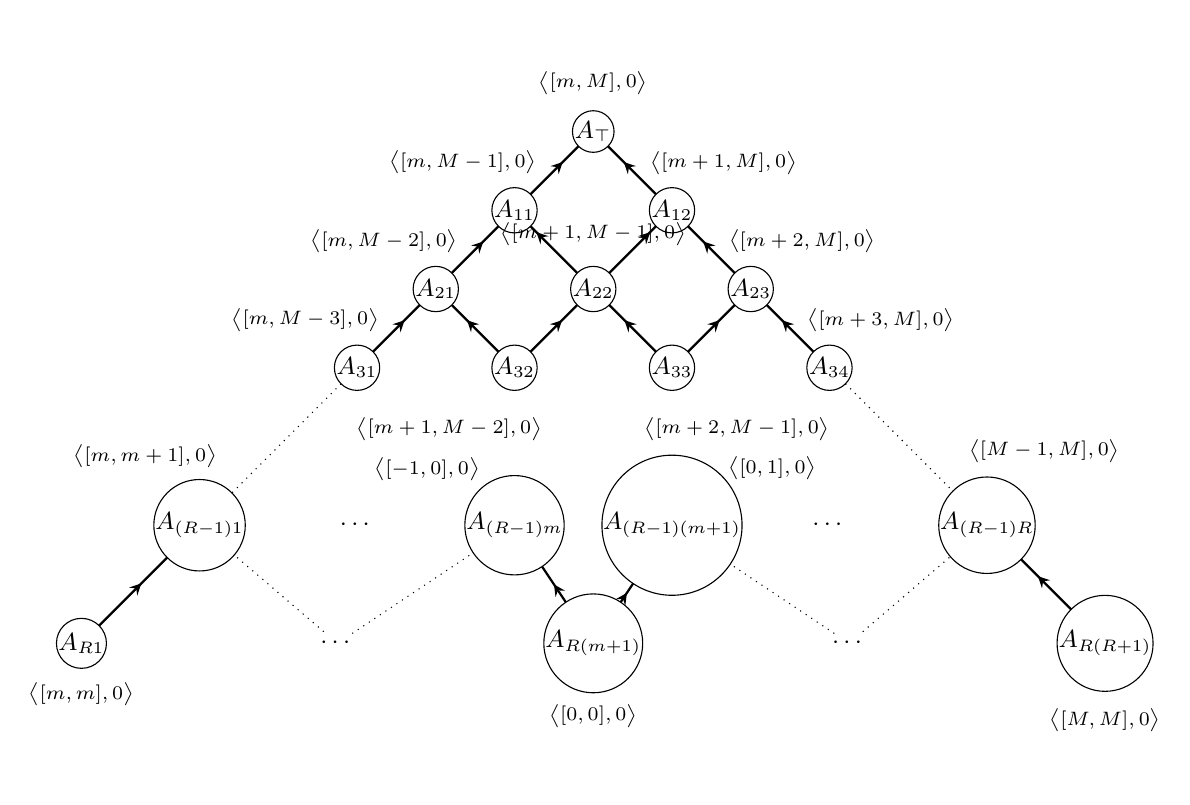
\begin{tikzpicture}[scale=0.5, every node/.style={draw, circle, inner sep=0pt, outer sep=0pt, font=\small}]
\newcommand\XRoot{12}
\newcommand\YRoot{12}
\node[label={[label distance=-10pt, font=\scriptsize]90:$\big<[m,M],0\big>$}] (Atop) at (\XRoot,\YRoot) {$A_\top$};
\node[label={[label distance=-10pt, font=\scriptsize]100:$\big<[m,M-1],0\big>$}] (A11) at (\XRoot-2,\YRoot-2) {$A_{11}$};
\node[label={[label distance=-10pt, font=\scriptsize]80:$\big<[m+1,M],0\big>$}] (A12) at (\XRoot+2,\YRoot-2) {$A_{12}$};
\node[label={[label distance=-10pt, font=\scriptsize]100:$\big<[m,M-2],0\big>$}] (A21) at (\XRoot-4,\YRoot-4) {$A_{21}$};
\node[label={[label distance=-22pt, font=\scriptsize]above:$\big<[m+1,M-1],0\big>$}] (A22) at (\XRoot,\YRoot-4) {$A_{22}$};
\node[label={[label distance=-10pt, font=\scriptsize]80:$\big<[m+2,M],0\big>$}] (A23) at (\XRoot+4,\YRoot-4) {$A_{23}$};
\node[label={[label distance=-10pt, font=\scriptsize]100:$\big<[m,M-3],0\big>$}] (A31) at (\XRoot-6,\YRoot-6) {$A_{31}$};
\node[label={[label distance=-10pt, font=\scriptsize]-100:$\big<[m+1,M-2],0\big>$}] (A32) at (\XRoot-2,\YRoot-6) {$A_{32}$};
\node[label={[label distance=-10pt, font=\scriptsize]-80:$\big<[m+2,M-1],0\big>$}] (A33) at (\XRoot+2,\YRoot-6) {$A_{33}$};
\node[label={[label distance=-10pt, font=\scriptsize]80:$\big<[m+3,M],0\big>$}] (A34) at (\XRoot+6,\YRoot-6) {$A_{34}$};
\node[label={[label distance=-10pt, font=\scriptsize]100:$\big<[m,m+1],0\big>$}] (All1) at (\XRoot-10,\YRoot-10) {$A_{(R-1)1}$};
\node[draw=none] at (\XRoot-6,\YRoot-10) {$\cdots$};
\node[label={[label distance=1pt, font=\scriptsize]-200:$\big<[-1,0],0\big>$}] (All2) at (\XRoot-2,\YRoot-10) {$A_{(R-1)m}$};
\node[label={[label distance=1pt, font=\scriptsize]20:$\big<[0,1],0\big>$}] (All3) at (\XRoot+2,\YRoot-10) {$A_{(R-1)(m+1)}$};
\node[draw=none] at (\XRoot+6,\YRoot-10) {$\cdots$};
\node[label={[label distance=-10pt, font=\scriptsize]80:$\big<[M-1,M],0\big>$}] (All4) at (\XRoot+10,\YRoot-10) {$A_{(R-1)R}$};
\node[label={[label distance=-10pt, font=\scriptsize]-90:$\big<[m,m],0\big>$}] (Al1) at (\XRoot-13,\YRoot-13) {$A_{R1}$};
\node[draw=none] (Al2) at (\XRoot-6.5,\YRoot-13) {$\cdots$};
\node[label={[label distance=-8pt, font=\scriptsize]-90:$\big<[0,0],0\big>$}] (Al3) at (\XRoot,\YRoot-13) {$A_{R(m+1)}$};
\node[draw=none] (Al4) at (\XRoot+6.5,\YRoot-13) {$\cdots$};
\node[label={[label distance=-10pt, font=\scriptsize]-90:$\big<[M,M],0\big>$}] (Al5) at (\XRoot+13,\YRoot-13) {$A_{R(R+1)}$};

\path (Atop) edge[-<-] (A11)
             edge[-<-] (A12)
      (A11)  edge[-<-] (A21)
             edge[-<-=0.3] (A22)
      (A12)  edge[-<-=0.3] (A22)
             edge[-<-] (A23)
      (A21)  edge[-<-] (A31)
             edge[-<-] (A32)
      (A22)  edge[-<-] (A32)
             edge[-<-] (A33)
      (A23)  edge[-<-] (A33)
             edge[-<-] (A34)
      (All1) edge[-<-] (Al1)
      (Al3)  edge[->-] (All2)
             edge[->-] (All3)
      (All4) edge[-<-] (Al5);
      
\path[dotted] (A31) edge (All1)
              (Al2) edge (All1)
                    edge (All2)
              (Al4) edge (All3)
                    edge (All4)
              (A34) edge (All4);
\end{tikzpicture}

\vspace{1cm}
\centerline{\underline{\Large{Frontal View}}}
\vspace{1cm}
\begin{description}
  \item[In the 2D Projectional View (Previous page):] \hfill
	\begin{itemize}
	  \item $m=\mathtt{MININT}$
	  \item $M=\mathtt{MAXINT}$
	  \item $0<\epsilon,\epsilon_1,\epsilon_2<1$
	  \item $\epsilon_2=\displaystyle\frac{\epsilon_1\cdot(M-m)}{M-m+1}\ \ \footnote{In general probability of an element = $\displaystyle\frac{\mathrm{(Probability\ of\ its\ direct\ parent)}\times\mathrm{(No.\ of\ elements\ in\ its\ own\ interval)}}{\mathrm{(No.\ of\ elements\ in\ its\ direct\ parent's\ interval)}}$}$
	\end{itemize}
  \item[In the Frontal \& Lateral View (Next page):] \hfill\\
    $A_{Ri}\equiv A_{(M-m)i}\quad\text{and}\quad\hat{A}_{Ri}\equiv\hat{A}_{(M-m)i}\qquad\forall i$\\
    For every pair of indices $i, j$ (and $\top$) the elements denoted by $A_{ij}$ (and $A_\top$) and $\hat{A}_{ij}$ (and $\hat{A}_\top$) have the same interval, but probability in element $A_{ij}$ (and $A_\top$) is $0$ , wherese it is 1 for $\hat{A}_{ij}$ (and $\hat{A}_\top$).\\
    E.g: $A_{22}\equiv\big<[m+1,\ M-1],\ 0\big>$ but $\hat{A}_{22}\equiv\big<[m+1,\ M-1],\ 1\big>$
\end{description}

\newpage
\begin{tikzpicture}[x={(6mm,-3.5mm)}, y={(0mm,15mm)}, z={(14mm,0mm)}, every node/.style={inner sep=2pt}, scale=0.9, remember picture, overlay, shift={(-20mm, -82mm)}]
\newcommand\Root{8}
\newcommand\Zoffset{8}
\newcommand\InitialBlack{0.7}
\node (A1) at (\Root,\Root,0) {$A_{\top}$};
\node (A2) at (\Root-1,\Root-1,0) {$A_{11}$};
\node (A3) at (\Root+1,\Root-1,0) {$A_{12}$};
\node (A4) at (\Root-2,\Root-2,0) {$A_{21}$};
\node (A5) at (\Root,\Root-2,0) {$A_{22}$};
\node (A6) at (\Root+2,\Root-2,0) {$A_{23}$};
\node (A7) at (\Root-3,\Root-3,0) {$A_{31}$};
\node (A8) at (\Root-1,\Root-3,0) {$A_{32}$};
\node (A9) at (\Root+1,\Root-3,0) {$A_{33}$};
\node (A10) at (\Root+3,\Root-3,0) {$A_{34}$};
\node (All1) at (\Root-5,\Root-5,0) {$A_{(R-1)1}$};
\node at (\Root-3,\Root-5,0) {$\ddots$};
\node (All2) at (\Root-1,\Root-5,0) {$A_{(R-1)m}$};
\node (All3) at (\Root+1,\Root-5,0) {$A_{(R-1)(m+1)}$};
\node at (\Root+3,\Root-5,0) {$\ddots$};
\node (All4) at (\Root+5,\Root-5,0) {$A_{(R-1)R}$};
\node (Al1) at (\Root-6,\Root-6,0) {$A_{R1}$};
\node (Al2) at (\Root-3,\Root-6,0) {$\ddots$};
\node (Al3) at (\Root,\Root-6,0) {$A_{R(m+1)}$};
\node (Al4) at (\Root+3,\Root-6,0) {$\ddots$};
\node (Al5) at (\Root+6,\Root-6,0) {$A_{R(R+1)}$};

\node (B1) at (\Root,\Root,\Zoffset) {$\hat{A}_{\top}$};
\node[lightgray] (B2) at (\Root-1,\Root-1,\Zoffset) {$\hat{A}_{11}$};
\node (B3) at (\Root+1,\Root-1,\Zoffset) {$\hat{A}_{12}$};
\node[lightgray] (B4) at (\Root-2,\Root-2,\Zoffset) {$\hat{A}_{21}$};
\node[inner sep=0pt] (B5) at (\Root,\Root-2,\Zoffset) {$\hat{A}_{22}$};
\node (B6) at (\Root+2,\Root-2,\Zoffset) {$\hat{A}_{23}$};
\node[lightgray] (B7) at (\Root-3,\Root-3,\Zoffset) {$\hat{A}_{31}$};
\node[lightgray] (B8) at (\Root-1,\Root-3,\Zoffset) {$\hat{A}_{32}$};
\node (B9) at (\Root+1,\Root-3,\Zoffset) {$\hat{A}_{33}$};
\node (B10) at (\Root+3,\Root-3,\Zoffset) {$\hat{A}_{34}$};
\node[lightgray] (Bll1) at (\Root-5,\Root-5,\Zoffset) {$\hat{A}_{(R-1)1}$};
\node[lightgray] (Bll2) at (\Root-1,\Root-5,\Zoffset) {$\hat{A}_{(R-1)m}$};
\node (Bll3) at (\Root+1,\Root-5,\Zoffset) {$\hat{A}_{(R-1)(m+1)}$};
\node (Bll4) at (\Root+5,\Root-5,\Zoffset) {$\hat{A}_{(R-1)R}$};
\node[lightgray] (Bl1) at (\Root-6,\Root-6,\Zoffset) {$\hat{A}_{R1}$};
\node[lightgray] (Bl2) at (\Root-3,\Root-6,\Zoffset) {$\ddots$};
\node (Bl3) at (\Root,\Root-6,\Zoffset) {$\hat{A}_{R(m+1)}$};
\node (Bl4) at (\Root+3,\Root-6,\Zoffset) {$\ddots$};
\node (Bl5) at (\Root+6,\Root-6,\Zoffset) {$\hat{A}_{R(R+1)}$};
\node (Bottom) at (\Root,\Root-8,\Zoffset) {$A_{\bot}$};

\path[dashed] (A1)   edge (B1)
              (A3)   edge[-<-=0.97] (B3)
              (A6)   edge[-<-=0.92] (B6)
              (A10)  edge[-<-=0.85] (B10)
              (All4) edge[-<-=0.9] (Bll4)
              (Al5)  edge[-<-=0.9] (Bl5);

\draw[dashed] (A2) -- (\Root-1,\Root-1,\InitialBlack) (A4) -- (\Root-2,\Root-2,\InitialBlack) (A5) -- (\Root,\Root-2,\InitialBlack) (A7) -- (\Root-3,\Root-3,\InitialBlack) (A8) -- (\Root-1,\Root-3,\InitialBlack) (A9) -- (\Root+1,\Root-3,\InitialBlack) (All1) -- (\Root-5,\Root-5,\InitialBlack*5) (All2) -- (\Root-1,\Root-5,\InitialBlack*3) (All3) -- (\Root+1,\Root-5,\InitialBlack*2) (Al1) -- (\Root-6,\Root-6,\InitialBlack*1.2) (Al3) -- (\Root,\Root-6,\InitialBlack*1.2);

\draw[lightgray, dashed] (\Root-1,\Root-1,\InitialBlack) -- (B2) (\Root-2,\Root-2,\InitialBlack) -- (B4) (\Root,\Root-2,\InitialBlack) -- (B5) (\Root-3,\Root-3,\InitialBlack) -- (B7) (\Root-1,\Root-3,\InitialBlack) -- (B8) (\Root+1,\Root-3,\InitialBlack) -- (\Root+1,\Root-3,\Zoffset-0.7) (\Root-5,\Root-5,\InitialBlack*5) -- (Bll1) (\Root-1,\Root-5,\InitialBlack*3) -- (Bll2) (\Root+1,\Root-5,\InitialBlack*2) -- (Bll3) (\Root-6,\Root-6,\InitialBlack*1.2) -- (Bl1) (\Root,\Root-6,\InitialBlack*1.2) -- (\Root,\Root-6,\Zoffset-0.8);

\draw[dashed] (\Root+1,\Root-3,\Zoffset-0.7) -- (B9) (\Root,\Root-6,\Zoffset-0.8) -- (Bl3);

\draw (A1) -- (A2) -- (A4) -- (A7) (A1) -- (A3) -- (A6) -- (A10);

\draw (A2) -- (A5) (A3) -- (A5) (A4) -- (A8) (A5) -- (A8) (A5) -- (A9) (A6) -- (A9) (All1) -- (Al1) (All4) -- (Al5) (All2) -- (Al3) (All3) -- (Al3) (Bl5) -- (Bottom) -- (\Root+6,\Root-5.5,\Zoffset*0.679) (Bottom) -- (\Root+5.75,\Root-5.78,\Zoffset*0.61);

\draw[dotted] (A7) -- (All1) -- (Al2) (A10) -- (All4) -- (Al4) (All2) -- (Al2) (All3) -- (Al4) (B10) -- (\Root+5,\Root-5,\Zoffset*0.6) (Bl2) -- (Bottom) -- (Bl4);

\draw (B1) edge[-<-=0.3] (\Root+1,\Root-1,\Zoffset*0.9) (B3) edge[-<-=0.2] (\Root+2,\Root-2,\Zoffset*0.8) (B6) edge[-<-=0.4] (\Root+3,\Root-3,\Zoffset*0.7) (Bll4) edge[-<-=0.4] (\Root+6,\Root-6,\Zoffset*0.5);

\draw[lightgray] (B1) edge[-<-] (\Root-1,\Root-1,\Zoffset*0.9) (B2) edge[-<-=0.2] (\Root,\Root-2,\Zoffset*0.8) (B2) edge[-<-=0.3] (\Root-2,\Root-2,\Zoffset*0.8) (B3) edge[-<-=0.4] (\Root,\Root-2,\Zoffset*0.8) (B4) edge[-<-=0.4] (\Root-3,\Root-3,\Zoffset*0.7) (B4) edge[-<-] (\Root-1,\Root-3,\Zoffset*0.7) (B5) edge[-<-=0.8] (\Root-1,\Root-3,\Zoffset*0.7) (B5) edge[-<-=0.7] (\Root+1,\Root-3,\Zoffset*0.7) (B6) edge[-<-=0.7] (\Root+1,\Root-3,\Zoffset*0.7) (Bll1) edge[-<-] (\Root-6,\Root-6,\Zoffset*0.5) (Bll2) edge[-<-=0.6] (\Root,\Root-6,\Zoffset*0.5) (Bll3) edge[-<-=0.6] (\Root,\Root-6,\Zoffset*0.5) (Bl3) edge[-<-] (\Root+6,\Root-5.5,\Zoffset*0.679) (\Root+5.75,\Root-5.78,\Zoffset*0.61) -- (Bl1);
\end{tikzpicture}
\\\\\\\\\\\\\\\\\\\\\\\\\\\\\\\\\\\\\\\\\\\\\\\\\\\\\\\\
\centerline{\underline{\Large{Lateral View (Skewed)}}}
\begin{tikzpicture}[remember picture, overlay, shift={(0mm, -90mm)}]
\newcommand\XRoot{8}
\newcommand\YRoot{8}
\node at (\XRoot,\YRoot) {$\hat{A}_\top$};
\node at (\XRoot-1,\YRoot-1) {$\hat{A}_{12}$};
\node at (\XRoot+1,\YRoot-1) {$\hat{A}_{11}$};
\node at (\XRoot-2,\YRoot-2) {$\hat{A}_{23}$};
\node at (\XRoot,\YRoot-2) {$\hat{A}_{22}$};
\node at (\XRoot+2,\YRoot-2) {$\hat{A}_{21}$};
\node[inner sep=15pt] (A34) at (\XRoot-3,\YRoot-3) {$\hat{A}_{34}$};
\node at (\XRoot-1,\YRoot-3) {$\hat{A}_{33}$};
\node at (\XRoot+1,\YRoot-3) {$\hat{A}_{32}$};
\node[inner sep=15pt] (A31) at (\XRoot+3,\YRoot-3) {$\hat{A}_{31}$};
\node[inner sep=15pt] (All6) at (\XRoot-5,\YRoot-5) {$\hat{A}_{(R-1)R}$};
\node at (\XRoot-3,\YRoot-5) {$\cdots$};
\node at (\XRoot-1,\YRoot-5) {$\hat{A}_{(R-1)(m+1)}$};
\node at (\XRoot+1,\YRoot-5) {$\hat{A}_{(R-1)m}$};
\node at (\XRoot+3,\YRoot-5) {$\cdots$};
\node[inner sep=15pt] (All1) at (\XRoot+5,\YRoot-5) {$\hat{A}_{(R-1)1}$};
\node (L1) at (\XRoot-6,\YRoot-6) {$\hat{A}_{R(R+1)}$};
\node (L2) at (\XRoot-3,\YRoot-6) {$\cdots$};
\node (L3) at (\XRoot,\YRoot-6) {$\hat{A}_{R(m+1)}$};
\node (L4) at (\XRoot+3,\YRoot-6) {$\cdots$};
\node (L5) at (\XRoot+6,\YRoot-6) {$\hat{A}_{R1}$};
\node (Bottom) at (\XRoot,\YRoot-8) {$A_\bot$};

\path (Bottom) edge[->-] (L1)
               edge[->-] (L3)
               edge[->-] (L5);

\draw[dotted] (L2) -- (Bottom) -- (L4) (A34) -- (All6) (A31) -- (All1);
\end{tikzpicture}
\\\\\\\\\\\\\\\\\\\\\\\\\\\\\\\\\\\\\\\\\\\\\\\\\\\\
\centerline{\underline{\Large{Rear View}}}






%% ------------------------------------------------------------
%%              References
%% ------------------------------------------------------------
 
\section*{References}
\bibliographystyle{plainnat}
\bibliography{references}

\end{document}
\endinput